% SI Section Two: Additional details on Machine Learning

\section{Additional details on machine learning method}

\subsection{d-band center and adsorption energy relations}
\label{supp_sec3.1_dband_eads}

% SI Figure 18: d-band venter vs adsorption energy scatter plot
\begin{figure}[htbp]
  \centering
  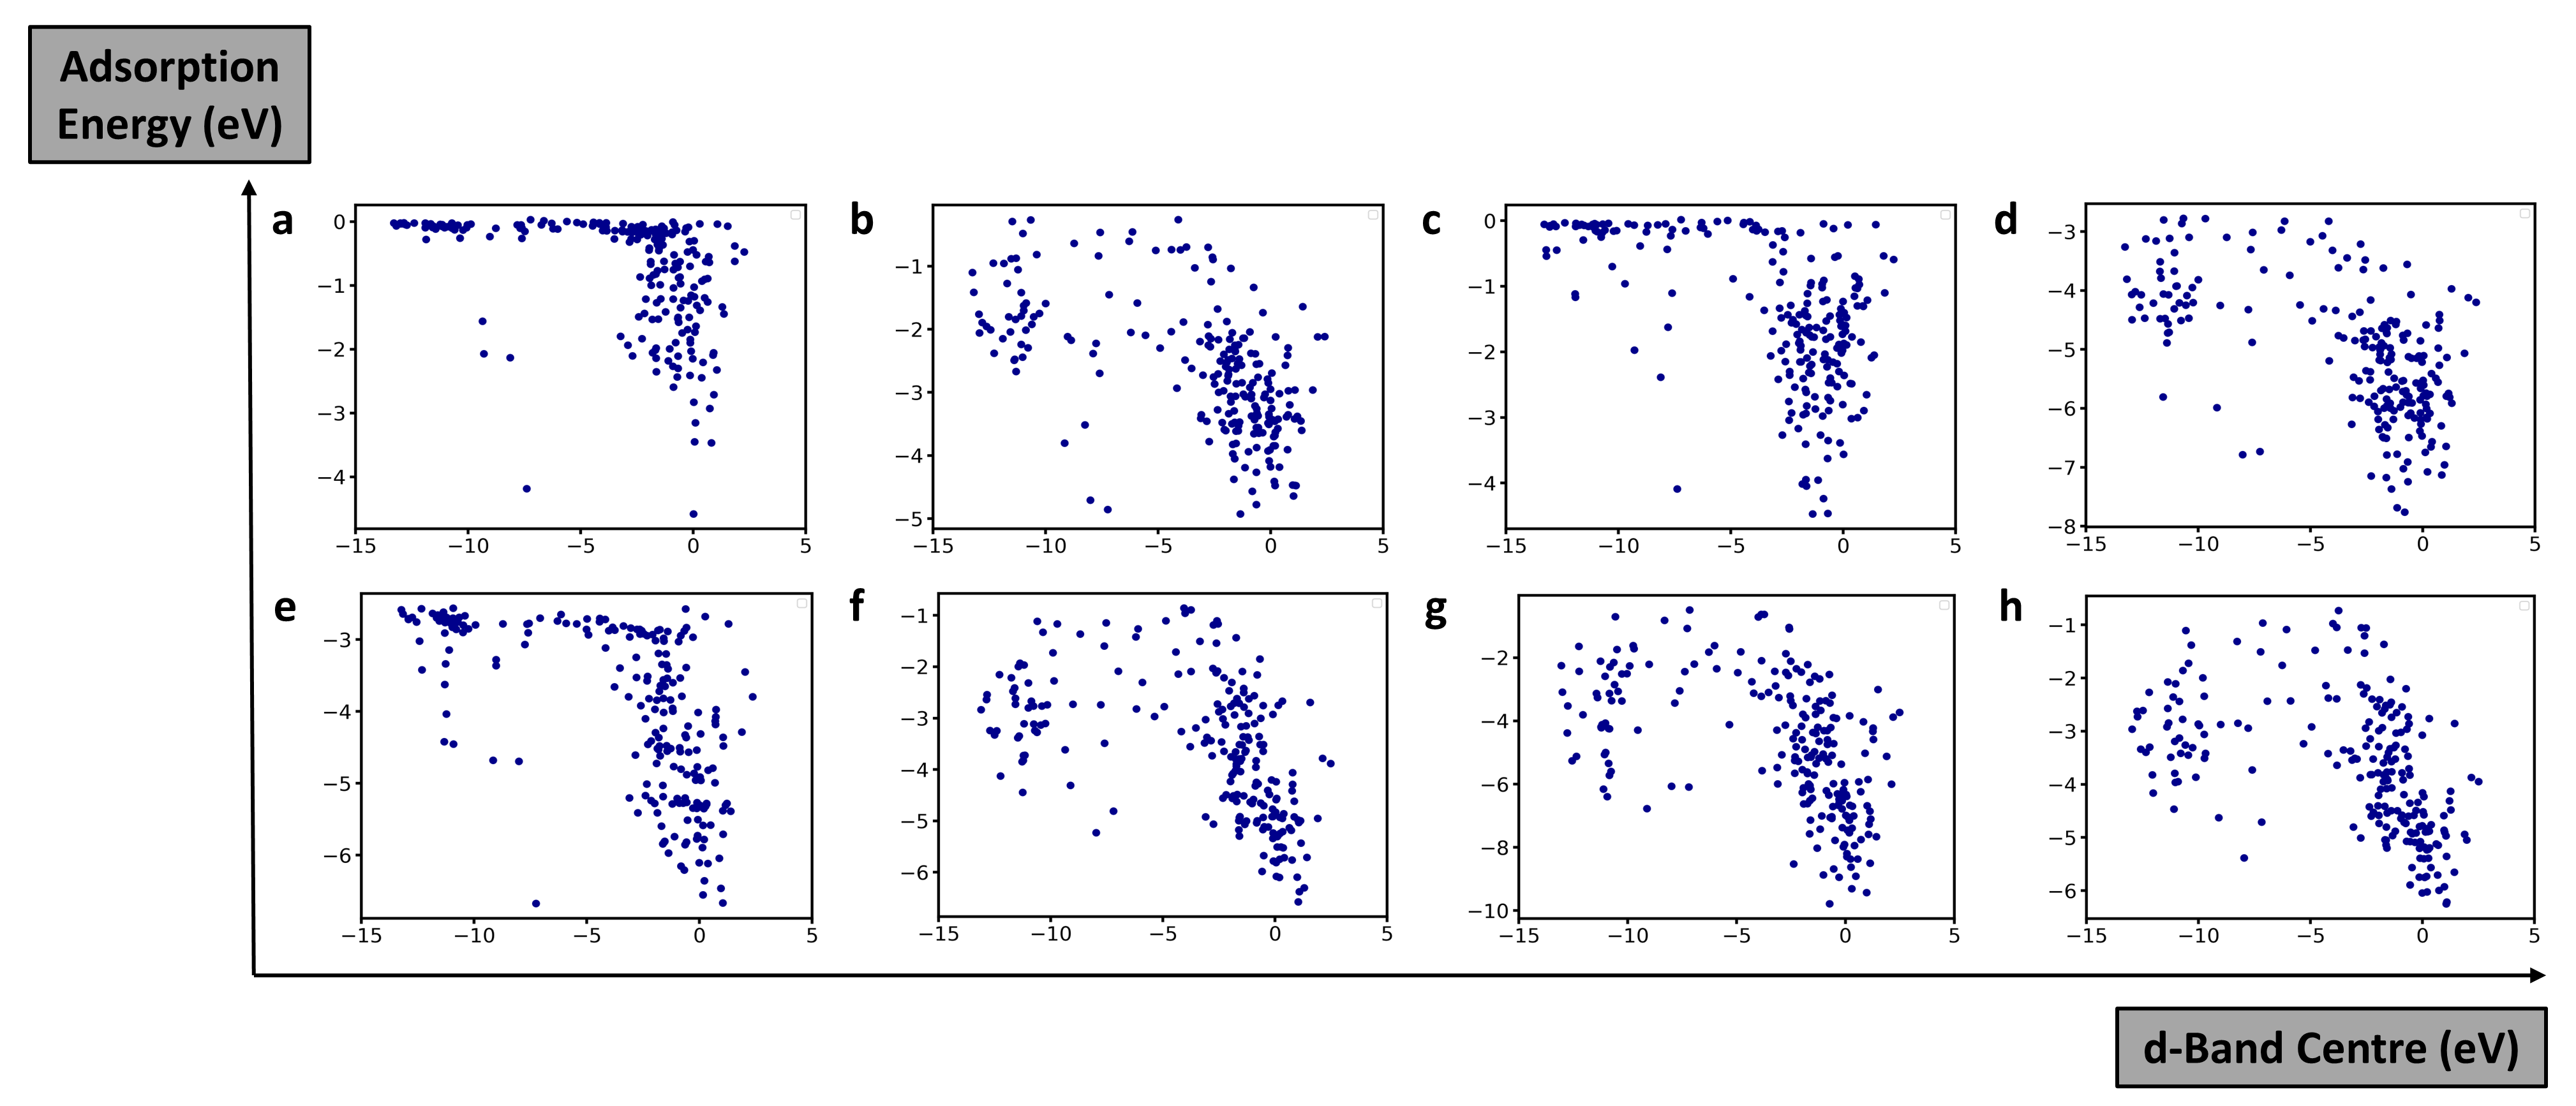
\includegraphics[width=\textwidth]{supp_fig18_d-band_eads.png}
  \caption{\textbf{Scatter plot of d-Band Center and Adsorption Energy Relationships.}
  This figure delineates the relationship between d-band center and adsorption energies for
  various species: (\textbf{a}) CO\textsubscript{2}, (\textbf{b}) COOH, (\textbf{c}) CO,
  (\textbf{d}) CHO, (\textbf{e}) CH\textsubscript{2}O, (\textbf{f}) OCH\textsubscript{3},
  (\textbf{g}) O, and (\textbf{h}) OH.
  Data from all six substrates investigated in this study are included.}
  \label{supp_fig18:dband_vs_eads}
\end{figure}

\subsection{Feature correlation analysis}
\label{supp_sec3.2_feature_corr}

\cref{supp_fig19:pairwise_eads_des} displays the pairwise relationships between CO adsorption energy
and its four most correlated descriptors: d-band center (spin-up) $\delta\epsilon_{\text{d}}\uparrow$,
lattice parameter $\gamma$, vacuum level $E_\text{vac}$, and electronegativity
on the Allen scale $\chi_\text{Allen}$, identified by Kendall rank correlation analysis.
\cref{supp_table15:descriptor_notations} lists notations for elementary descriptors and electronic descriptors.

% SI Figure 19: Pairwise plot of adsorption energy vs key descriptors
\begin{figure}[htbp]
  \centering
  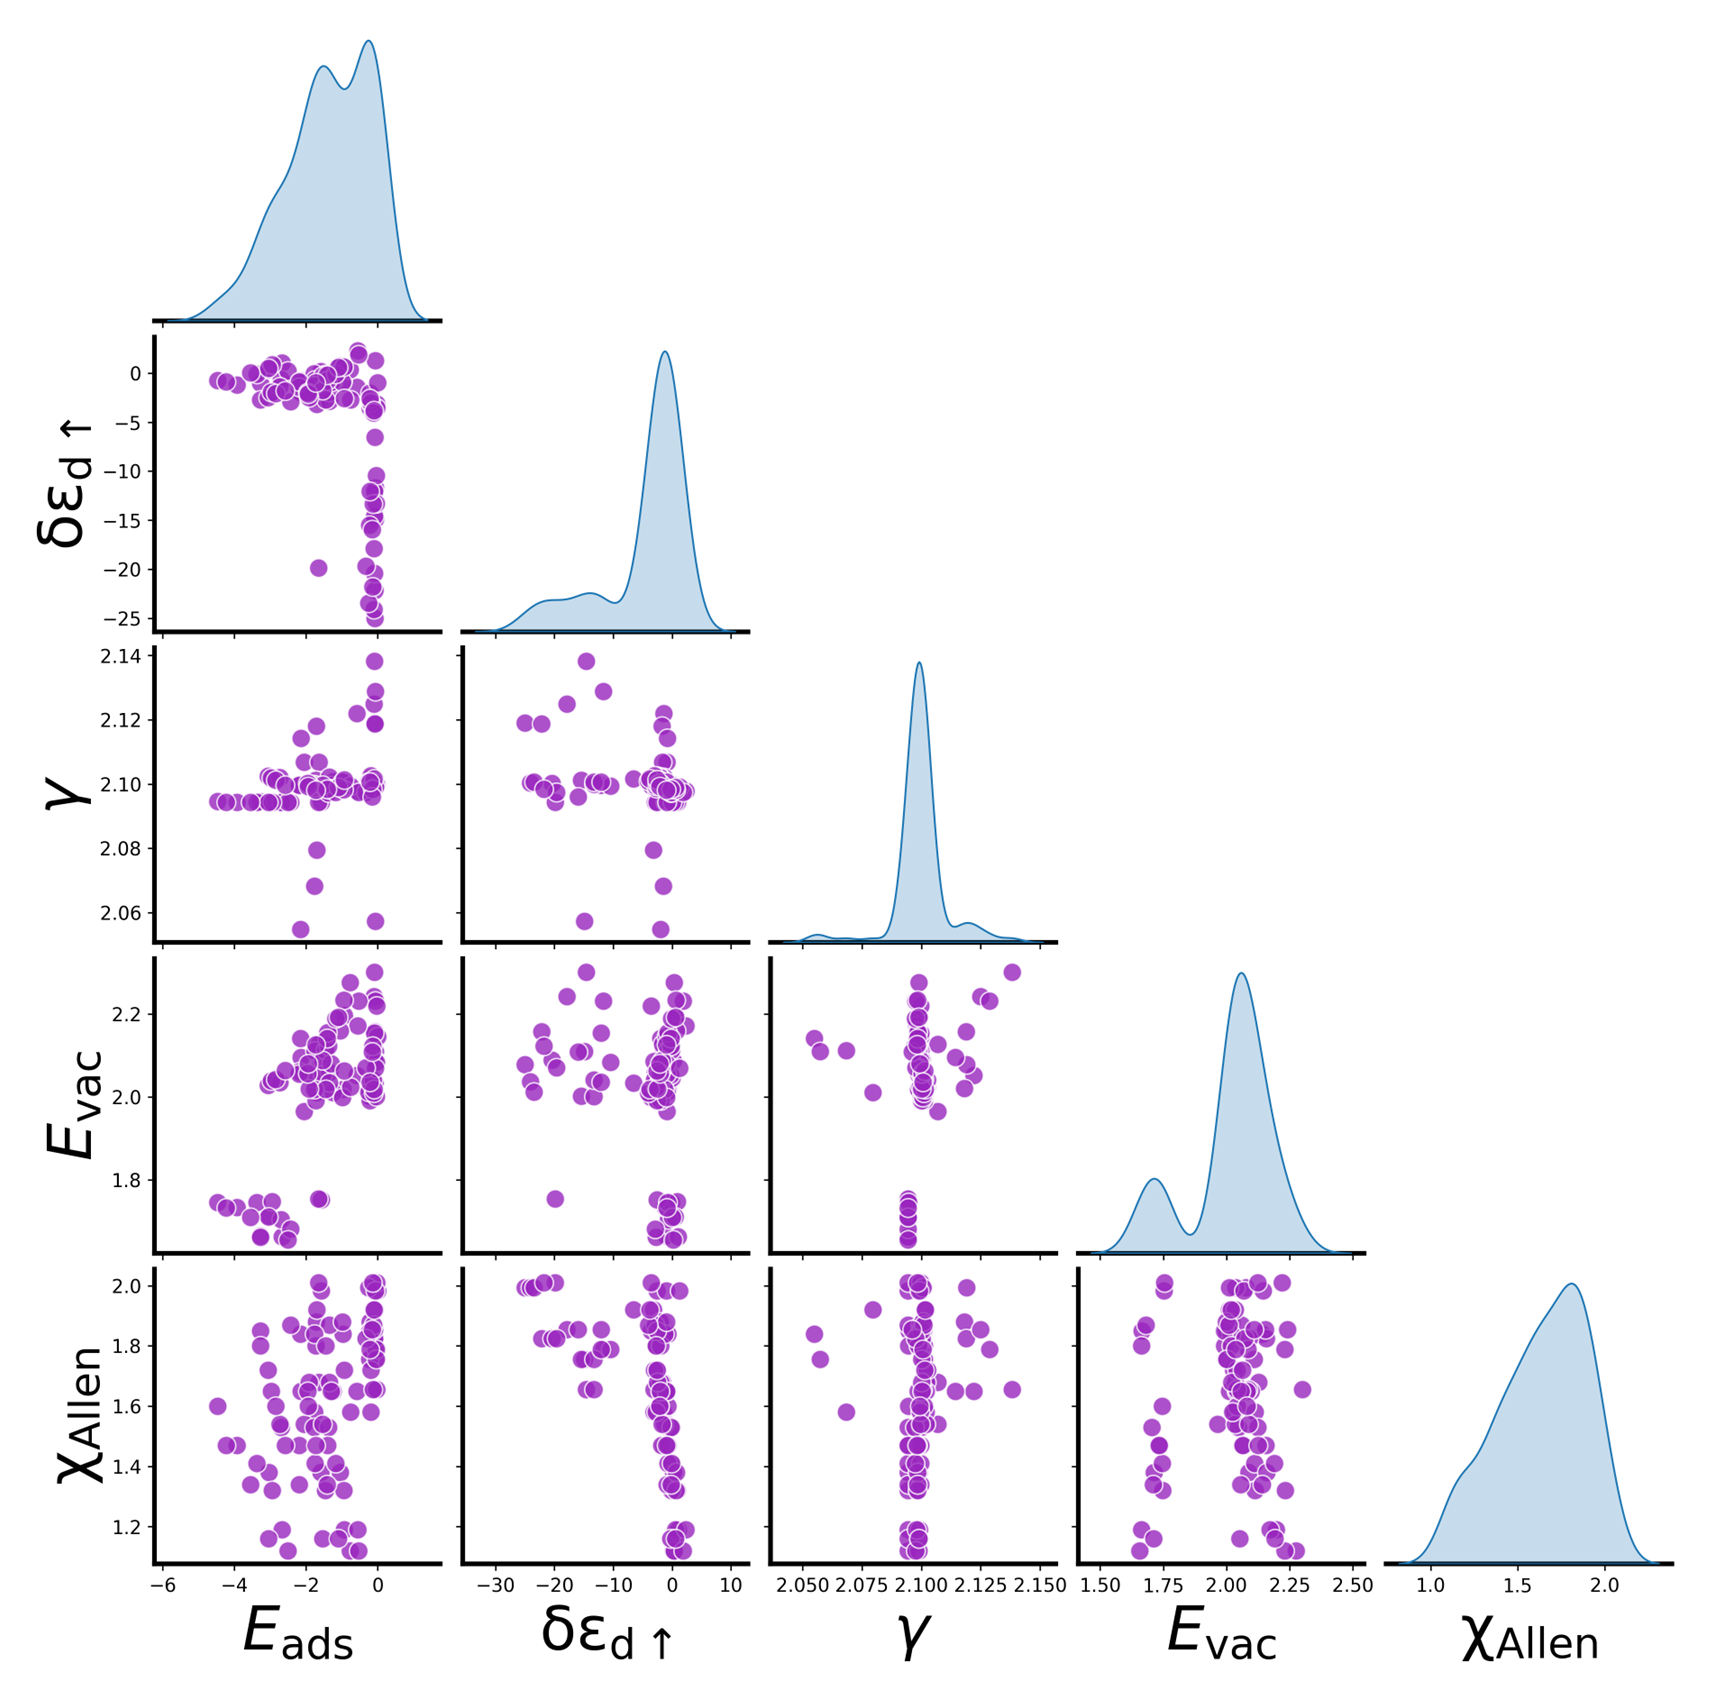
\includegraphics[width=\textwidth]{supp_fig19_pairwise_eads_des.png}
  \caption{\textbf{Pairwise Plot of Adsorption Energy and Key Descriptors.}
  This chart displays the pairwise relationships between CO adsorption energy and
  its four most correlated descriptors: d-band center (spin-up) $\delta\epsilon_{\text{d}}\uparrow$,
  lattice parameter $\gamma$, vacuum level $E_\text{vac}$, and electronegativity
  on the Allen scale $\chi_\text{Allen}$, identified by Kendall rank correlation analysis.
  Data from all six substrates investigated in this study are included.}
  \label{supp_fig19:pairwise_eads_des}
\end{figure}

% Supplementary Table 15: Notations for elementary descriptors and electronic descriptors
\begin{table}[htbp]
\label{supp_table15:descriptor_notations}
  \caption{Notations for elementary descriptors and electronic descriptors.}
  \resizebox{\textwidth}{!}{%
    \begin{tabular}{llll}
      \toprule
      \multicolumn{2}{c}{Elementary Descriptors}       & \multicolumn{2}{c}{Electronic Descriptors}            \\
      \midrule
      $R$            & atomic radius                   & $\alpha$, $\beta$, $\gamma$  & lattice parameters     \\
      $E_\text{ea}$  & electron affinity               & $\Phi_{\text{DFT}}$    & DFT calculated work function \\
      $\Phi$         & work function                   & $E_\text{vac}$         & vacuum level                 \\
      $\chi_\text{Allen}$, $\chi_\text{P}$, $\chi_\text{RevP}$
      & \parbox[t]{4cm}{electronegativity in Allen, Pauling and revised Pauling scales}
      & $E_\text{g}$, $E_\text{g}\uparrow$, $E_\text{g}\uparrow$
      & \parbox[t]{4cm}{average, spin-up and spin-down band gaps}                                              \\
      $A_\text{r}$   & relative atomic mass            & $e_\text{d}$           & number of d-electrons        \\
      $E_\text{i}$   & ionization energy & $\delta\epsilon_{\text{d}}\uparrow$  & d-band centre (spin-up)      \\
      $G$            & group number                    & $W_\text{d}$           & d-band width                 \\
      $P$            & period number                   & $e_{\text{Bader}}$     & Bader charge                 \\
      $V$            & number of valence electrons     &                        &                              \\
      \bottomrule
    \end{tabular}
  }
\end{table}

\subsection{Input pipeline construction}
\label{supp_sec3.3_input_pipeline}

The format of the 2D array for the eDOS is naturally well-suited for use as neural network inputs.
In this study, the array adopts a shape of [numSamplings, numOrbitals, numChannels], as illustrated in \cref{supp_fig20:input_dos}.
Here, ``numSamplings'' represents the number of data points sampled across the energy spectrum,
``numOrbitals'' denotes the number of DOS orbitals,
and ``numChannels'' indicates the number of atomic channels.

% SI Figure 20: Representation of the input eDOS data structure
\begin{figure}[htbp]
  \centering
  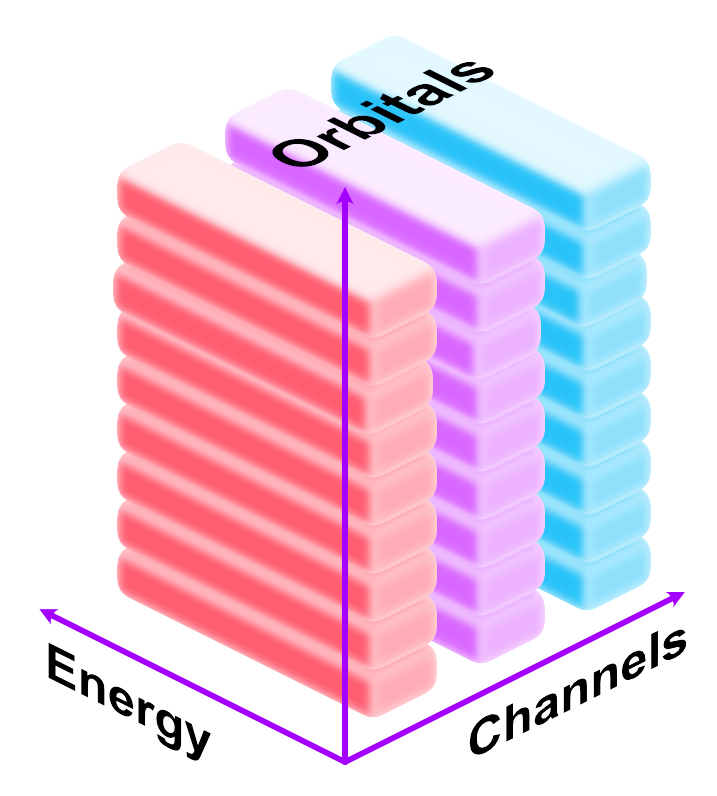
\includegraphics[width=0.3\textwidth]{supp_fig20_input_dos.png}
  \caption{\textbf{Schematic representation of the input eDOS data structure.}}
  \label{supp_fig20:input_dos}
\end{figure}

For practical purposes, certain spatial hierarchies are expected to remain invariant,
such as the energy range over which the eDOS is sampled.
In this work, we maintain a consistent energy range of -14 eV to 6 eV,
sampled at a density of 50 \si{\text{points} \cdot \text{eV}^{-1}}.
In addition to maintaining a fixed energy range,
the following steps are taken to standardize the input eDOS data:
  1.	For atoms lacking d-electrons, the eDOS is zero-padded.
  2.	f-orbital eDOS data are excluded.
  3.	The eDOS of adsorbates is zero-padded along the Channels axis to align with the adsorbate that contains the maximum number of atoms, which, in this study, is the *OCH\textsubscript{3} species. This padded eDOS is then appended to the metal eDOS.

As a result of these preprocessing steps, the input eDOS arrays consistently have a shape of [4000, 9, 6].
This corresponds to 4000 sampling points across the energy range, 9 eDOS orbitals, and 6 atomic channels.

\subsection{Hyperparameter tuning for CNN}
\label{supp_sec3.4_hyperparam}

% Supplementary Table 16: The hyperparameter search space
\begin{table}[htbp]
\label{supp_table16:hyperparam_space}
  \caption{The hyperparameter search space.}
  \resizebox{\textwidth}{!}{%
    \begin{tabular}{lll}
      \toprule
      Hyperparameter& Search Space              & Description                                                       \\
      \midrule
      learningRate  & [10\textsuperscript{-4}, 10\textsuperscript{-2}], log scale & Learning rate of Adam \cite{kingma2017adam} optimizer \\
      dropoutRate   & [0, 1]                    & Dropout rate                                                      \\
      root\_fc0     & 128, 256, 512             & Output dimensionality of 1\textsuperscript{st} fully connected layer in root           \\
      root\_fc1     & 256, 512, 1024, 2048      & Output dimensionality of 2\textsuperscript{nd} fully connected layer in root           \\
      root\_act     & ``tanh'', ``relu'', ``sigmoid'' & Activation function of fully connected layers in root             \\
      kernelSize    & [2, 32]                   & Width of the convolution window                                   \\
      numFilters    & [8, 64]                   & Number of filters in the convolution                              \\
      numConvLayers & [1, 16]                   & Number of convolution layers                                      \\
      numConvBlocks & [1, 16]                   & Number of convolution blocks                                      \\
      br\_fc0       & 16, 32, 64, 128, 256, 512 & Output dimensionality of 1\textsuperscript{st} fully connected layer in branch      \\
      br\_fc1       & 8, 16, 32, 64, 128, 256   & Output dimensionality of 2\textsuperscript{nd} fully connected layer in branch      \\
      br\_act       & ``tanh'', ``relu'', ``sigmoid'' & Activation function of fully connected layers in branch           \\
      \bottomrule
    \end{tabular}
  }
\end{table}

% Supplementary Table 17: Optimal hyperparameters identified with Hyperband algorithm
\begin{table}[htbp]
\label{supp_table17:opt_hyperparam}
  \caption{Optimal hyperparameters identified with Hyperband algorithm.}
  \resizebox{\textwidth}{!}{%
    \begin{tabular}{lll}
      \toprule
      Hyperparameter& Optimal Value & Description                                              \\
      \midrule
      learningRate  & $10^{-3}$ & Learning rate of Adam \cite{kingma2017adam} optimizer                              \\
      dropoutRate   & 0.3       & Dropout rate                                                 \\
      root\_fc0     & 256       & Output dimensionality of 1\textsuperscript{st} fully connected layer in root   \\
      root\_fc1     & 512       & Output dimensionality of 2\textsuperscript{nd} fully connected layer in root   \\
      root\_act     & ``relu''    & Activation function of fully connected layers in root        \\
      kernelSize    & 10        & Width of convolution window                                  \\
      numFilters    & 17        & Number of filters in the convolution                         \\
      numConvLayers & 3         & Number of convolution layers                                 \\
      numConvBlocks & 1         & Number of convolution blocks                                 \\
      br\_fc0       & 256       & Output dimensionality of 1\textsuperscript{st} fully connected layer in branch \\
      br\_fc1       & 128       & Output dimensionality of 2\textsuperscript{nd} fully connected layer in branch \\
      br\_act       & ``tanh''    & Activation function of fully connected layers in branch      \\
      \bottomrule
    \end{tabular}
  }
\end{table}

% Supplementary Table 18: Prediction MAEs of the CNN model
\begin{table}[htbp]
\label{supp_table18:cnn_mae}
  \caption{Prediction mean absolute errors of the CNN model.}
  \small
  \begin{tabularx}{\textwidth}{@{}lXX@{}}
    \toprule
    Adsorbate             & Original dataset (eV)  & Augmented dataset (eV)  \\
    \midrule
    CO\textsubscript{2}   & 0.0447                 & 0.0336                  \\
    COOH                  & 0.0436                 & 0.0581                  \\
    CO                    & 0.0402                 & 0.0402                  \\
    CHO                   & 0.0614                 & 0.0778                  \\
    CH\textsubscript{2}O  & 0.0553                 & 0.0632                  \\
    OCH\textsubscript{3}  & 0.0605                 & 0.0636                  \\
    O                     & 0.1135                 & 0.1081                  \\
    OH                    & 0.0547                 & 0.0602                  \\
    H                     & 0.0703                 & 0.0646                  \\
    \bottomrule
  \end{tabularx}

  \smallskip

  \footnotesize\textit{Note:} The same CNN model, trained on the
    augmented dataset, was used for all predictions. The term ``original dataset''
    refers to evaluations conducted on the original dataset without any augmented data;
    it does not imply the use of a different CNN model trained solely on the original dataset.
    Similarly, ``augmented dataset'' refers to evaluations on the dataset with
    both original data and augment data, not a distinct model.
\end{table}

\subsection{Occlusion experiment}
\label{supp_sec3.5_occlusion}

% SI Figure 21: Illustration of the eDOS occlusion experiment
\begin{figure}[htbp]
  \centering
  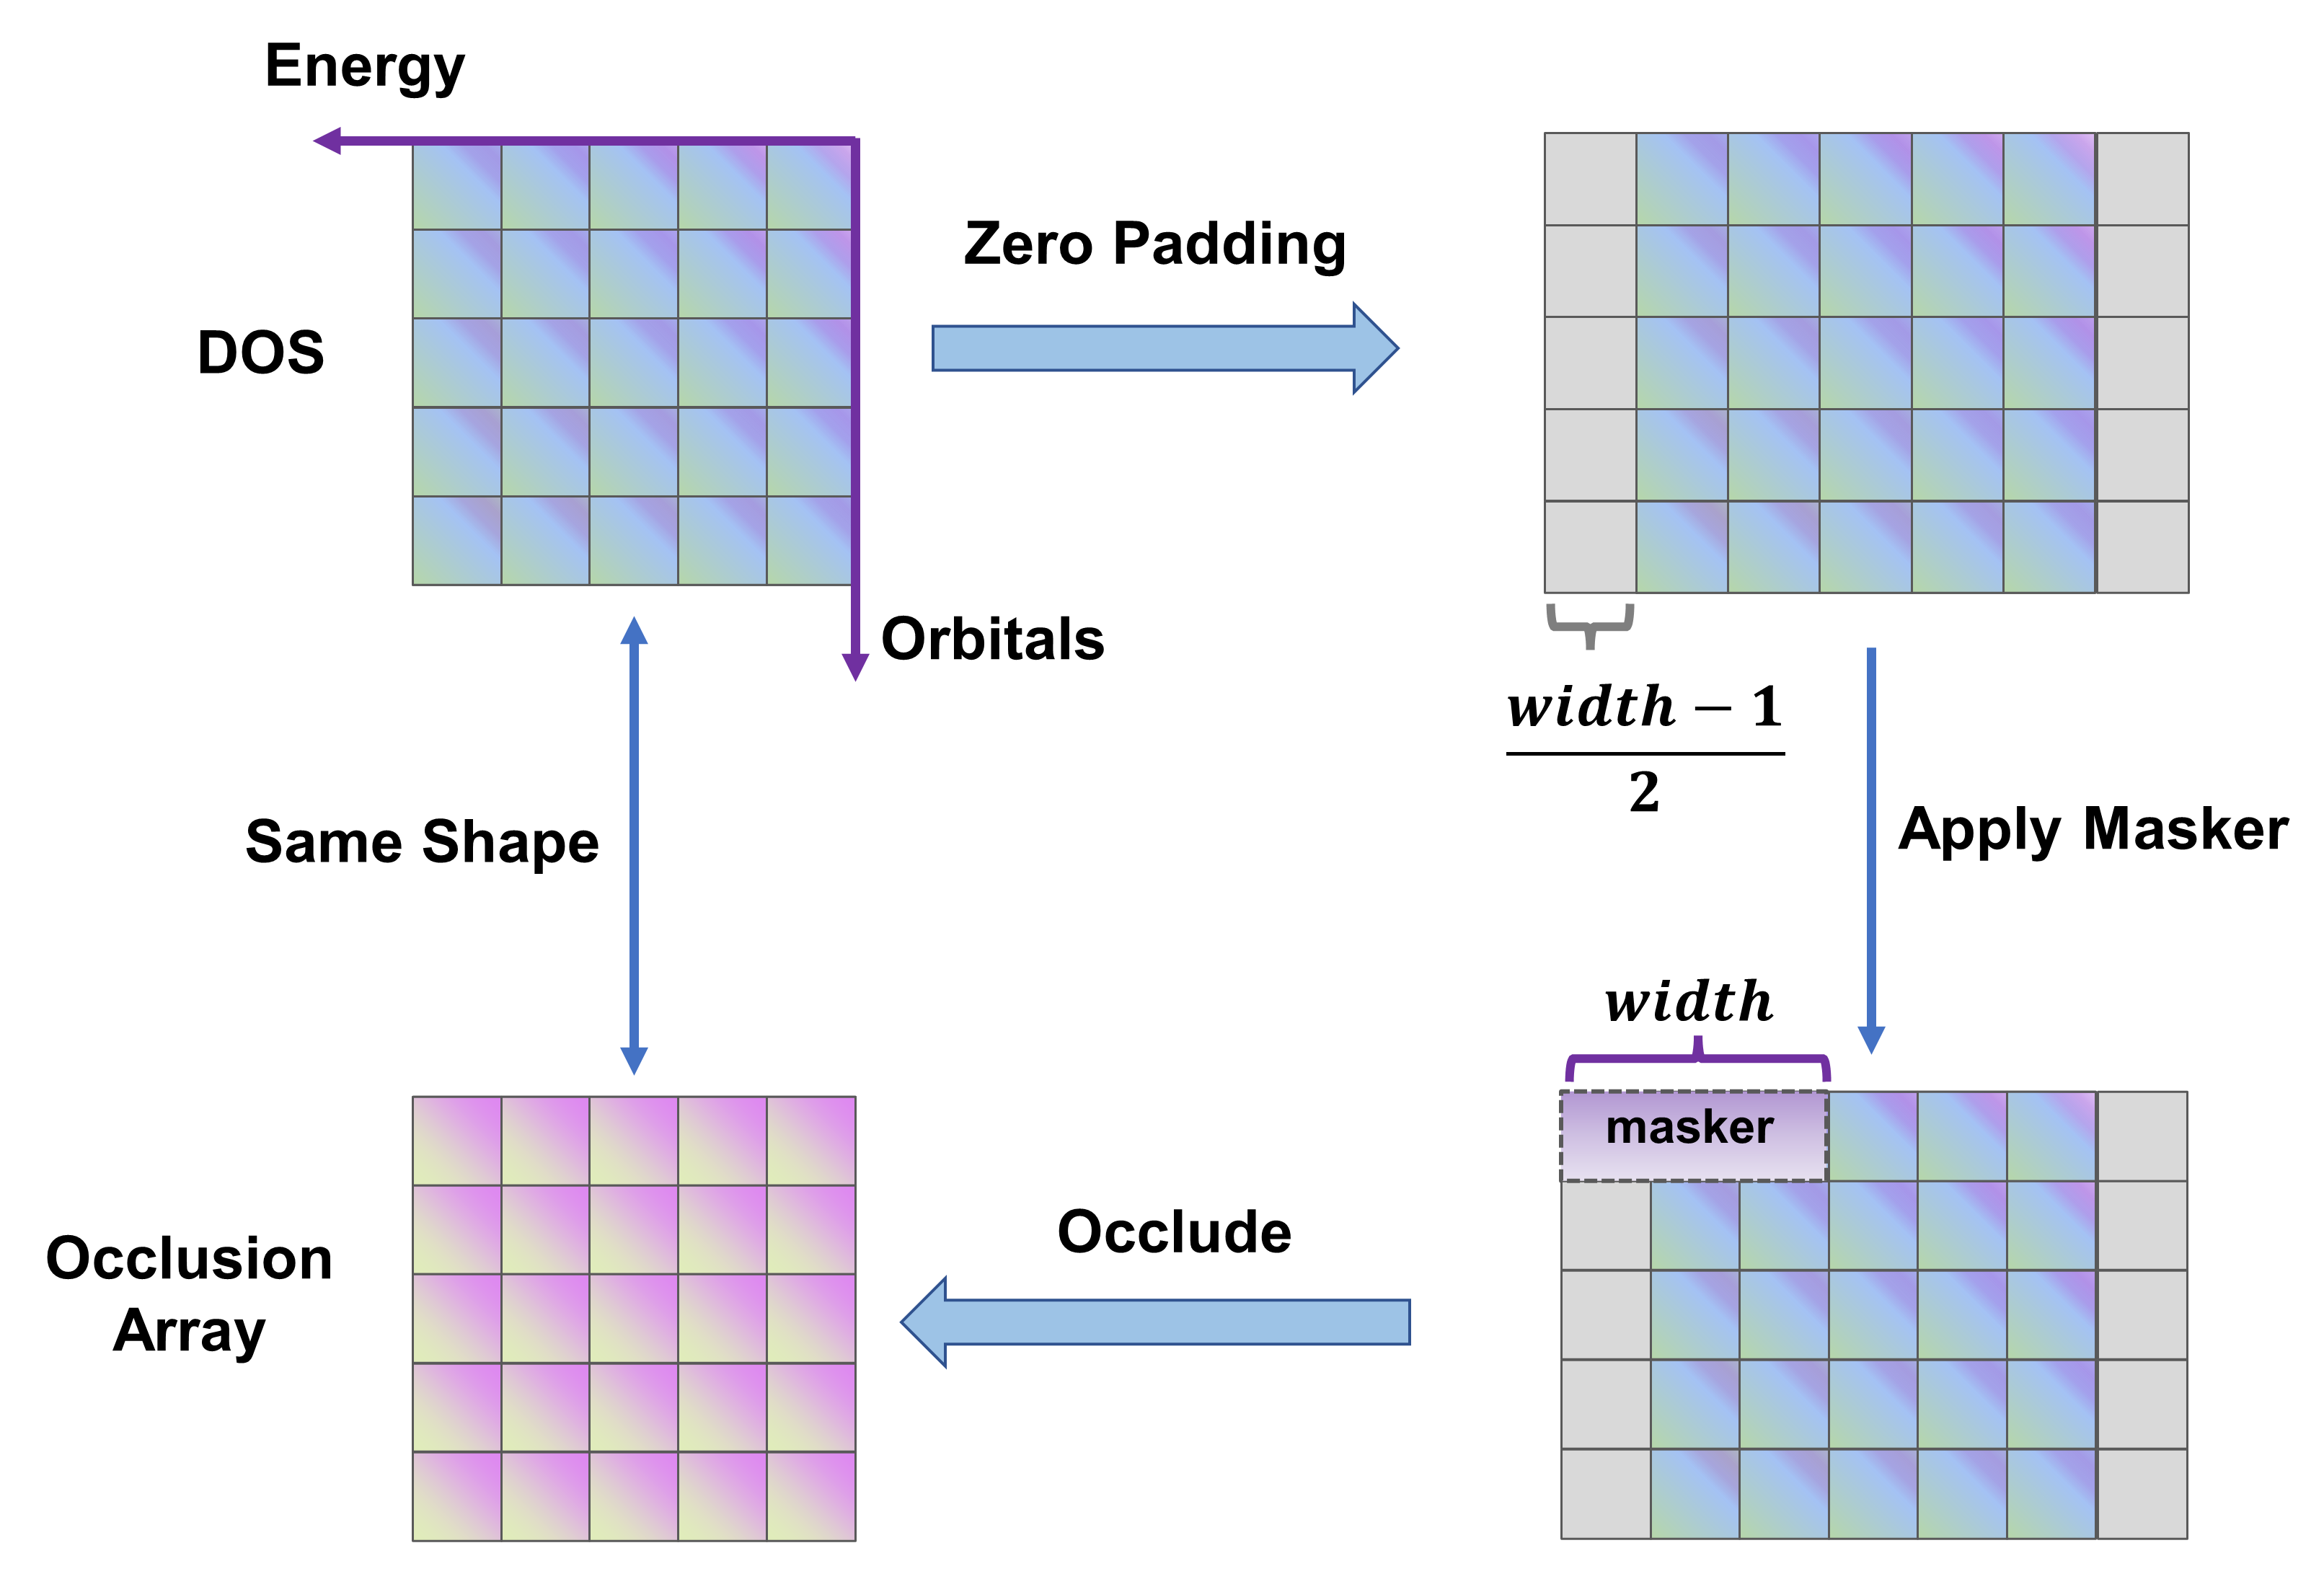
\includegraphics[width=\textwidth]{supp_fig21_occlusion.png}
  \caption{\textbf{Illustration of the eDOS occlusion experiment.}
  This figure demonstrates the step-by-step process of the occlusion experiment.
  The input eDOS array first undergoes zero-padded, and then a masker of width ``width'' is applied,
  resulting in an occlusion array that preserves the shape of the input array.}
  \label{supp_fig21:occlusion}
\end{figure}

% SI Figure 22: Occlusion experiment with a masker width of 1
\begin{figure}[htbp]
  \centering
  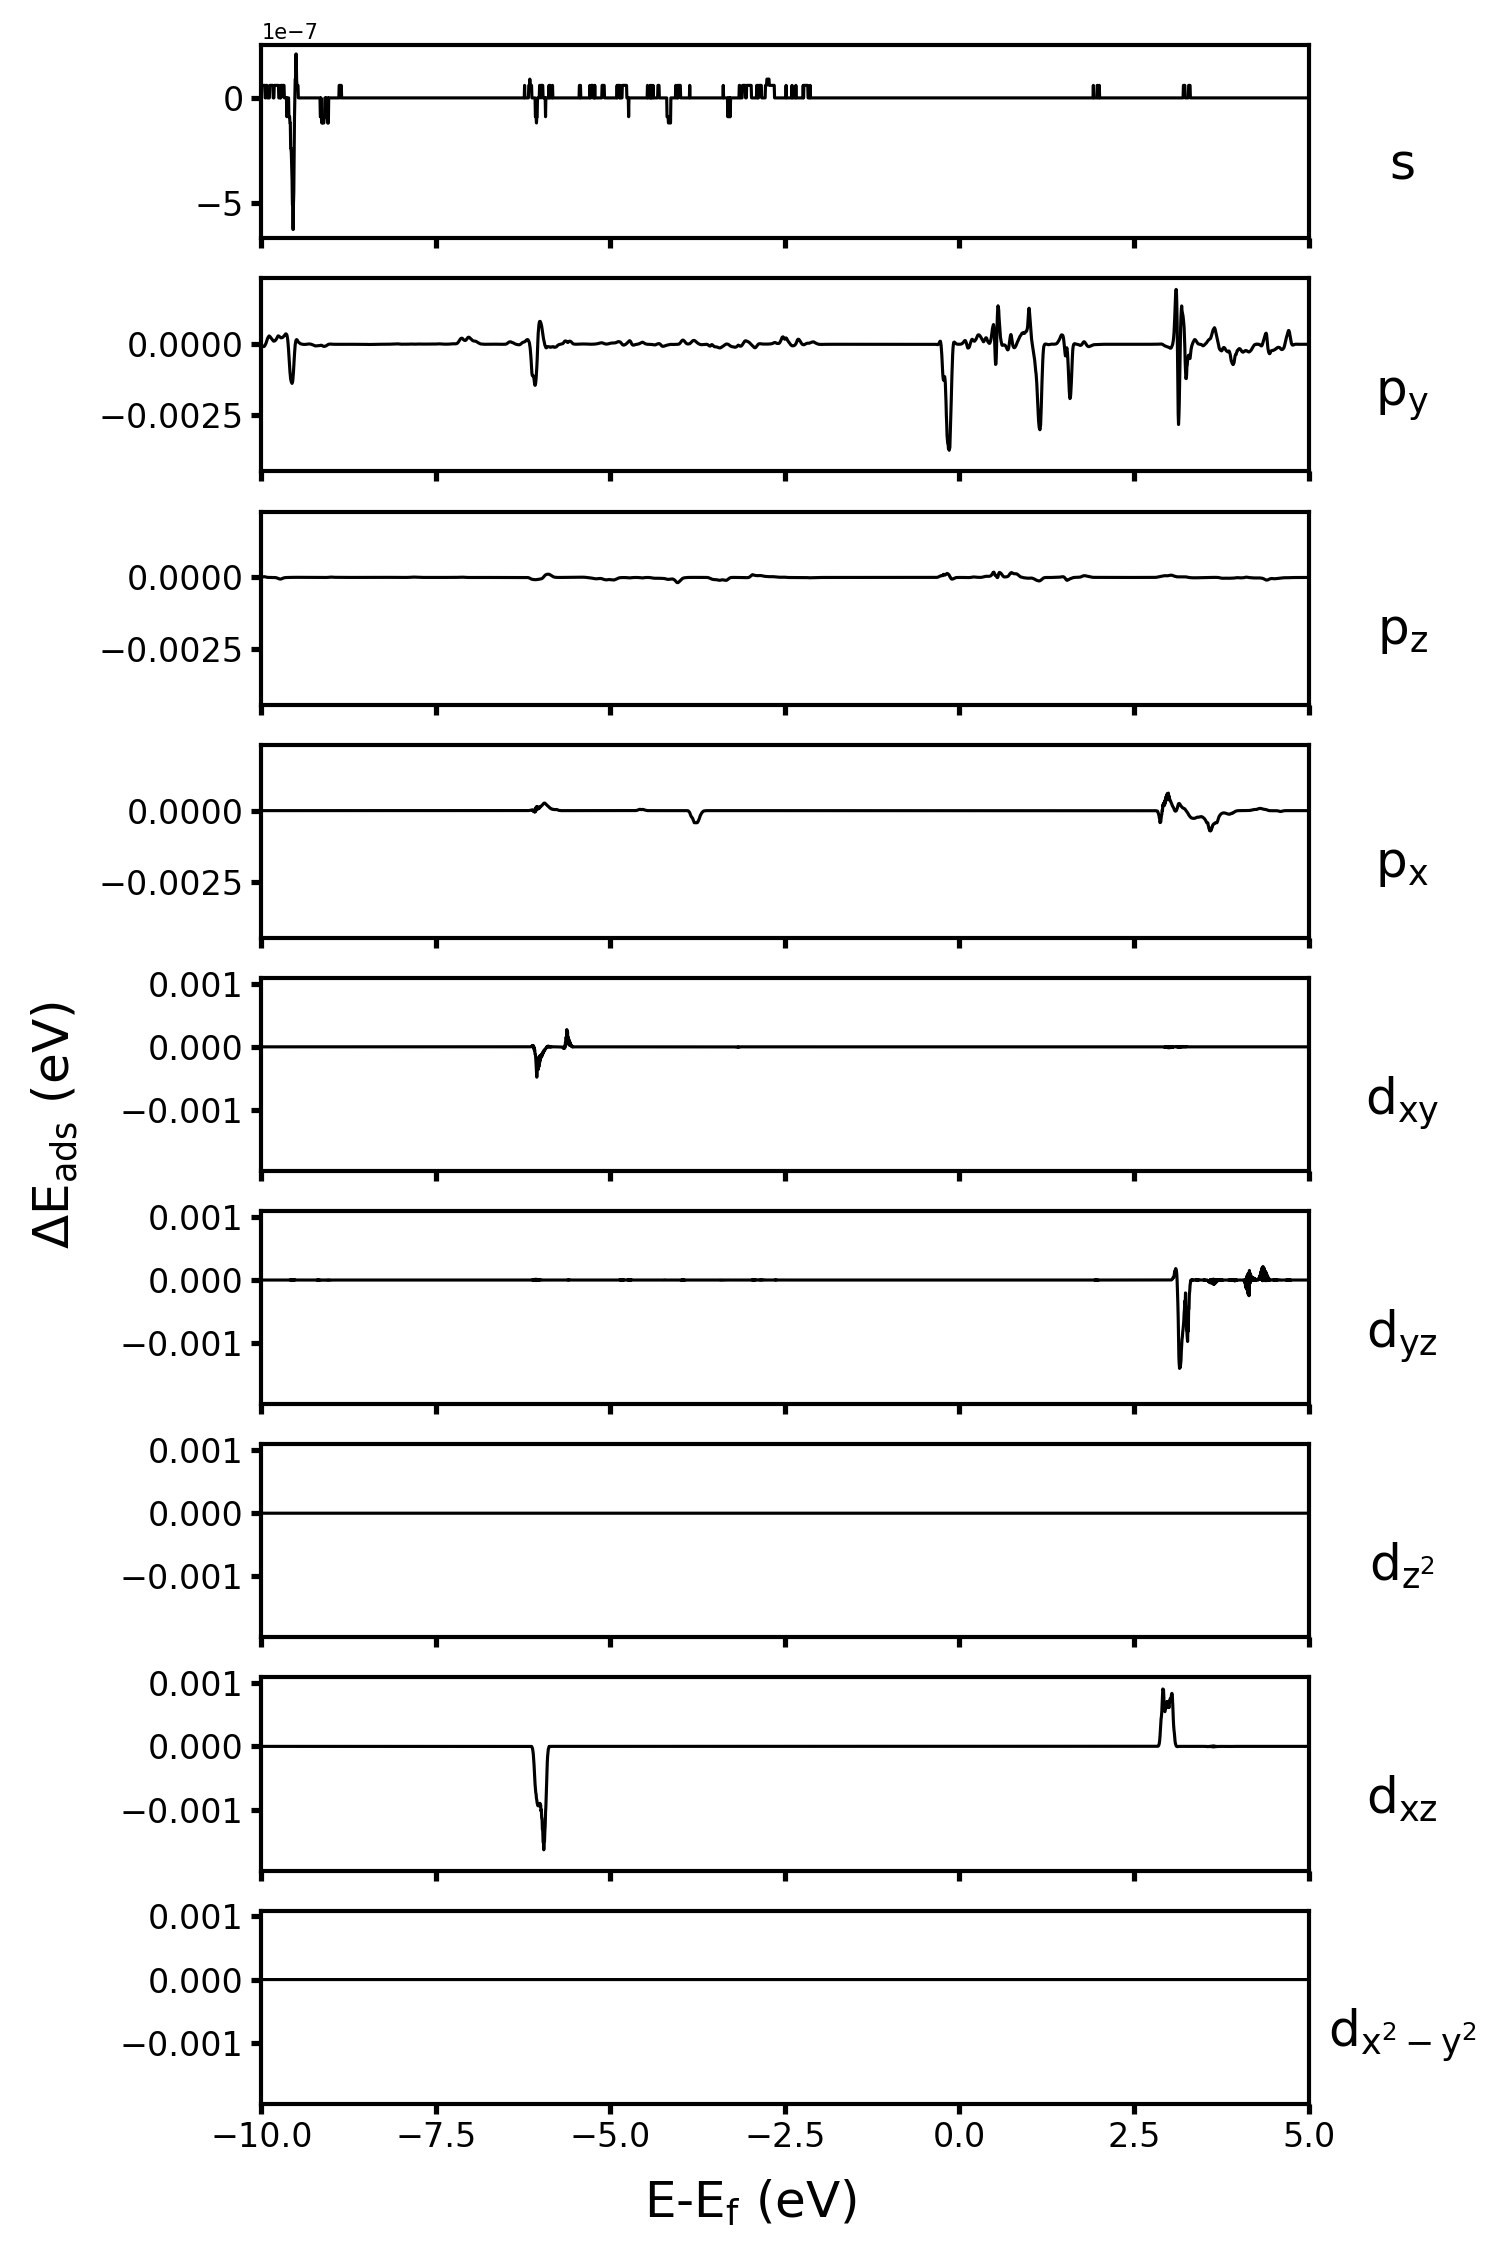
\includegraphics[width=0.6\textwidth]{supp_fig22_occl_wid1.png}
  \caption{\textbf{Occlusion Experiment with a masker width of ``1''.}
  This figure shows an occlusion experiment on the Ge atom in
  the initial state of CO adsorption on Ge@g-C\textsubscript{3}N\textsubscript{4}.}
  \label{supp_fig22:occl_wid1}
\end{figure}

% SI Figure 23: Occlusion experiment with a masker width of 3
\begin{figure}[htbp]
  \centering
  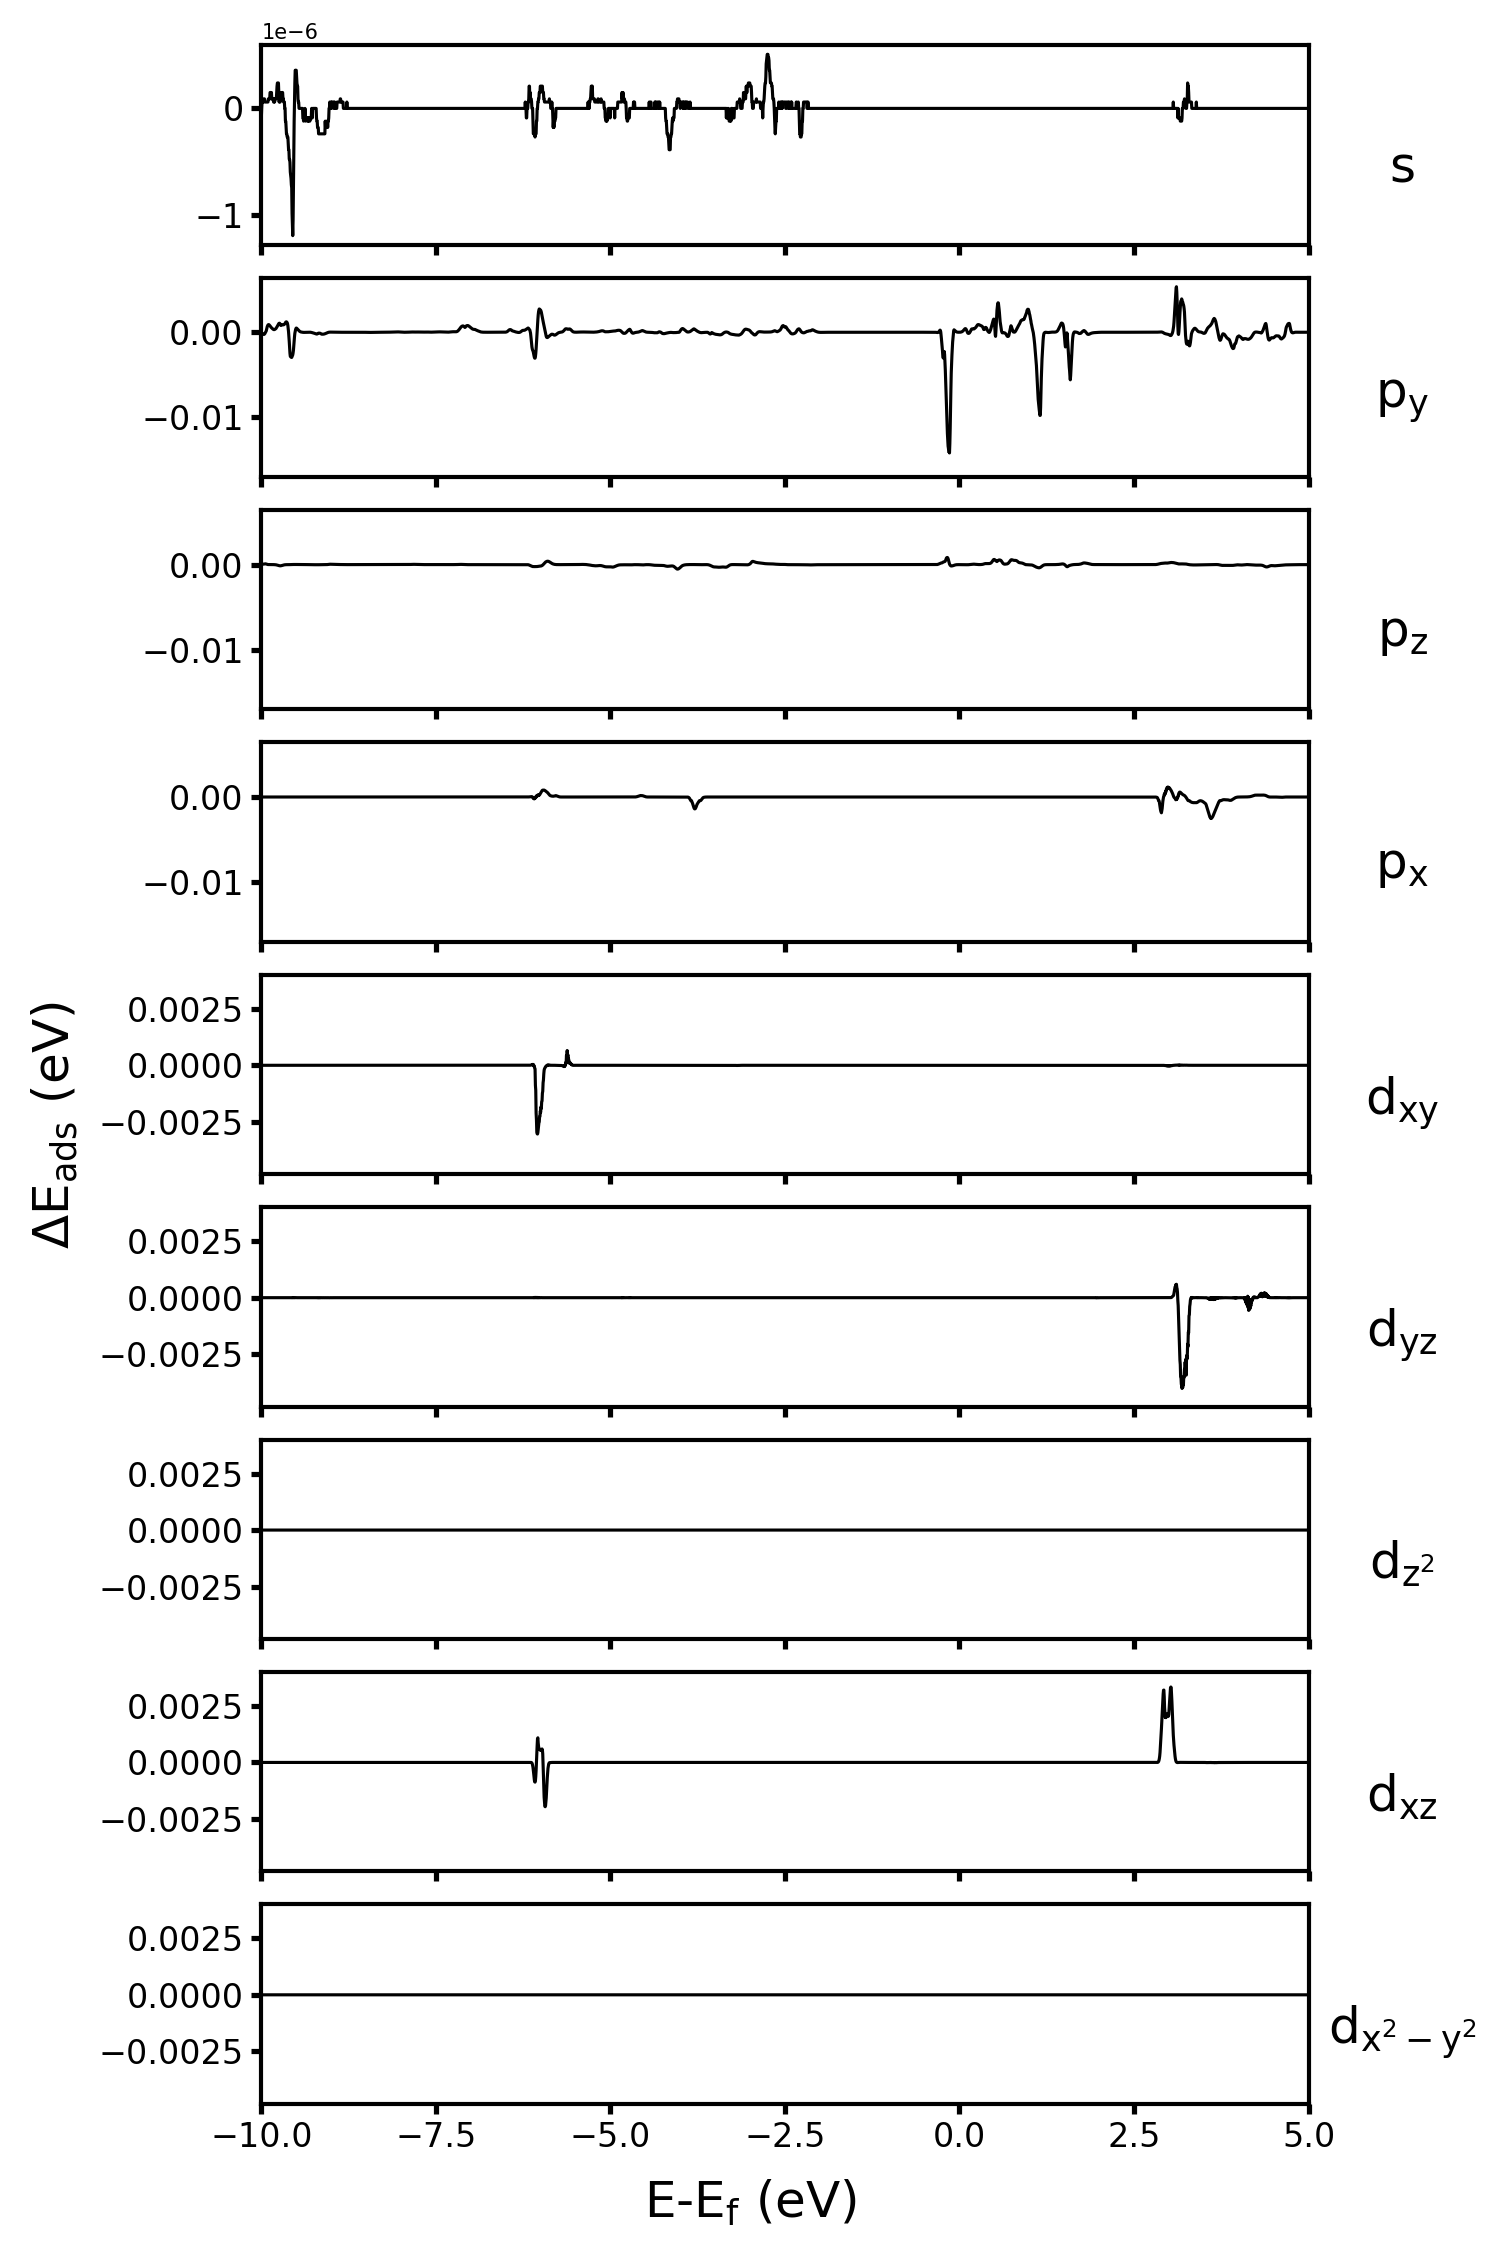
\includegraphics[width=0.6\textwidth]{supp_fig23_occl_wid3.png}
  \caption{\textbf{Occlusion Experiment with a masker width of ``3''.}
  This figure shows an occlusion experiment on the Ge atom in
  the initial state of CO adsorption on Ge@g-C\textsubscript{3}N\textsubscript{4}.}
  \label{supp_fig23:occl_wid3}
\end{figure}

% SI Figure 24: Occlusion experiment with a masker width of 5
\begin{figure}[htbp]
  \centering
  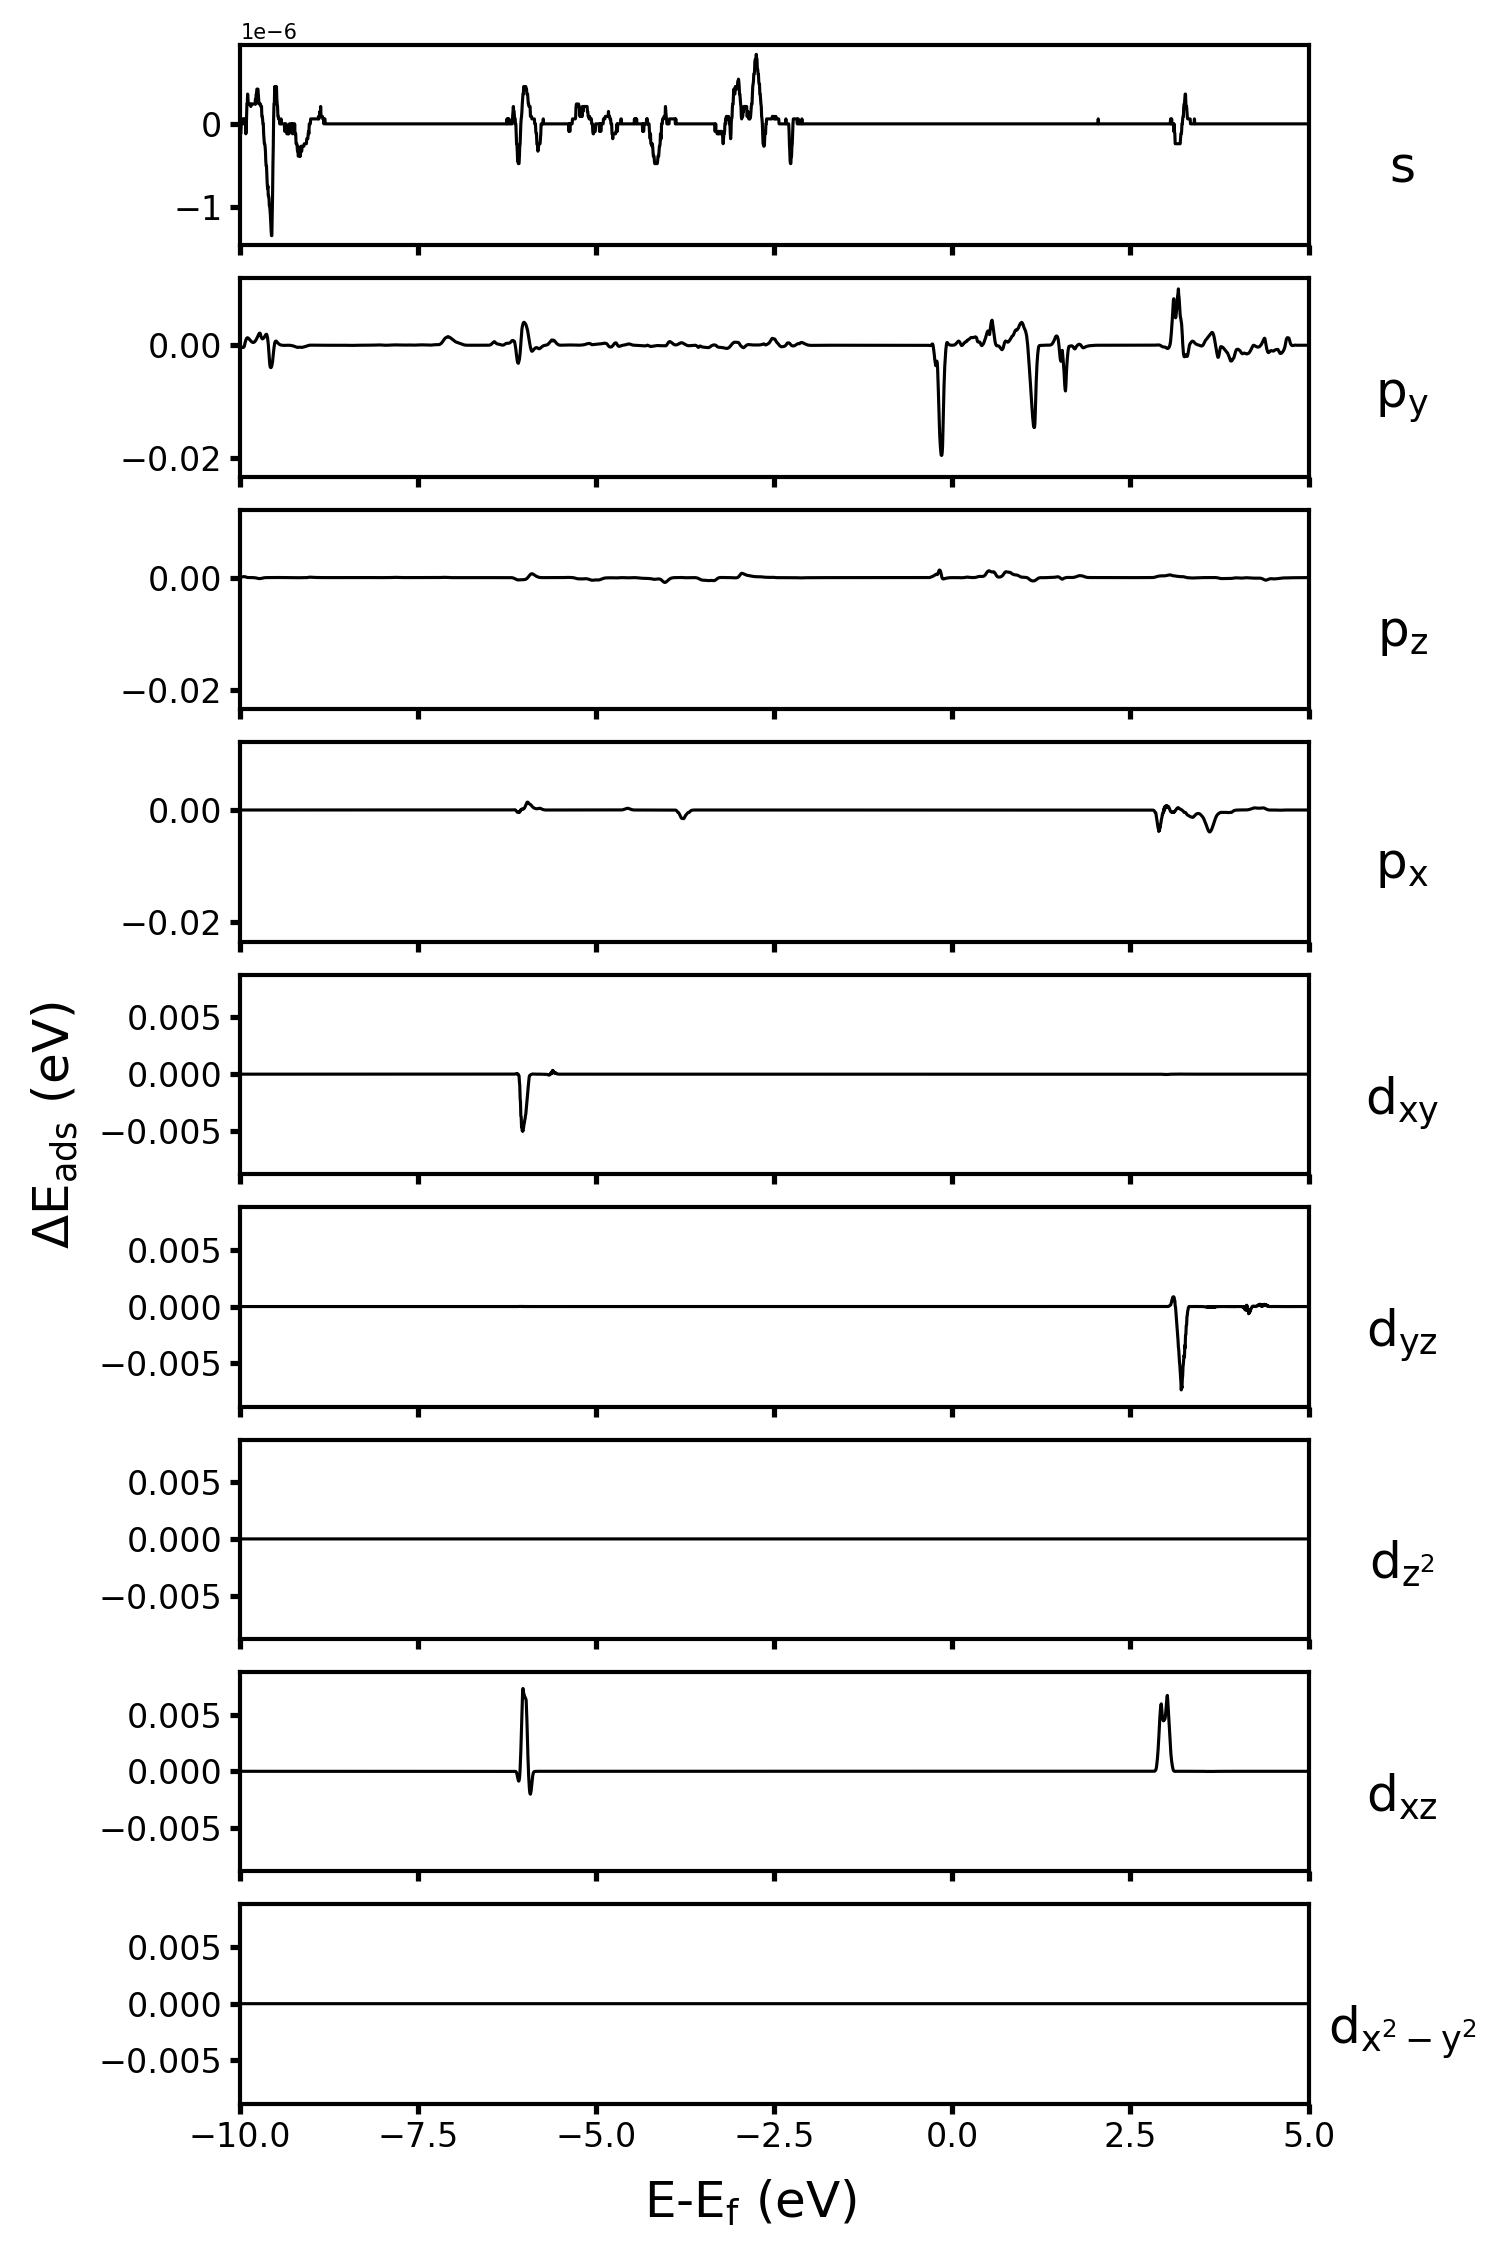
\includegraphics[width=0.6\textwidth]{supp_fig24_occl_wid5.png}
  \caption{\textbf{Occlusion Experiment with a masker width of ``5''.}
  This figure shows an occlusion experiment on the Ge atom in
  the initial state of CO adsorption on Ge@g-C\textsubscript{3}N\textsubscript{4}.}
  \label{supp_fig24:occl_wid5}
\end{figure}

% SI Figure 25: Occlusion experiment with a masker width of 11
\begin{figure}[htbp]
  \centering
  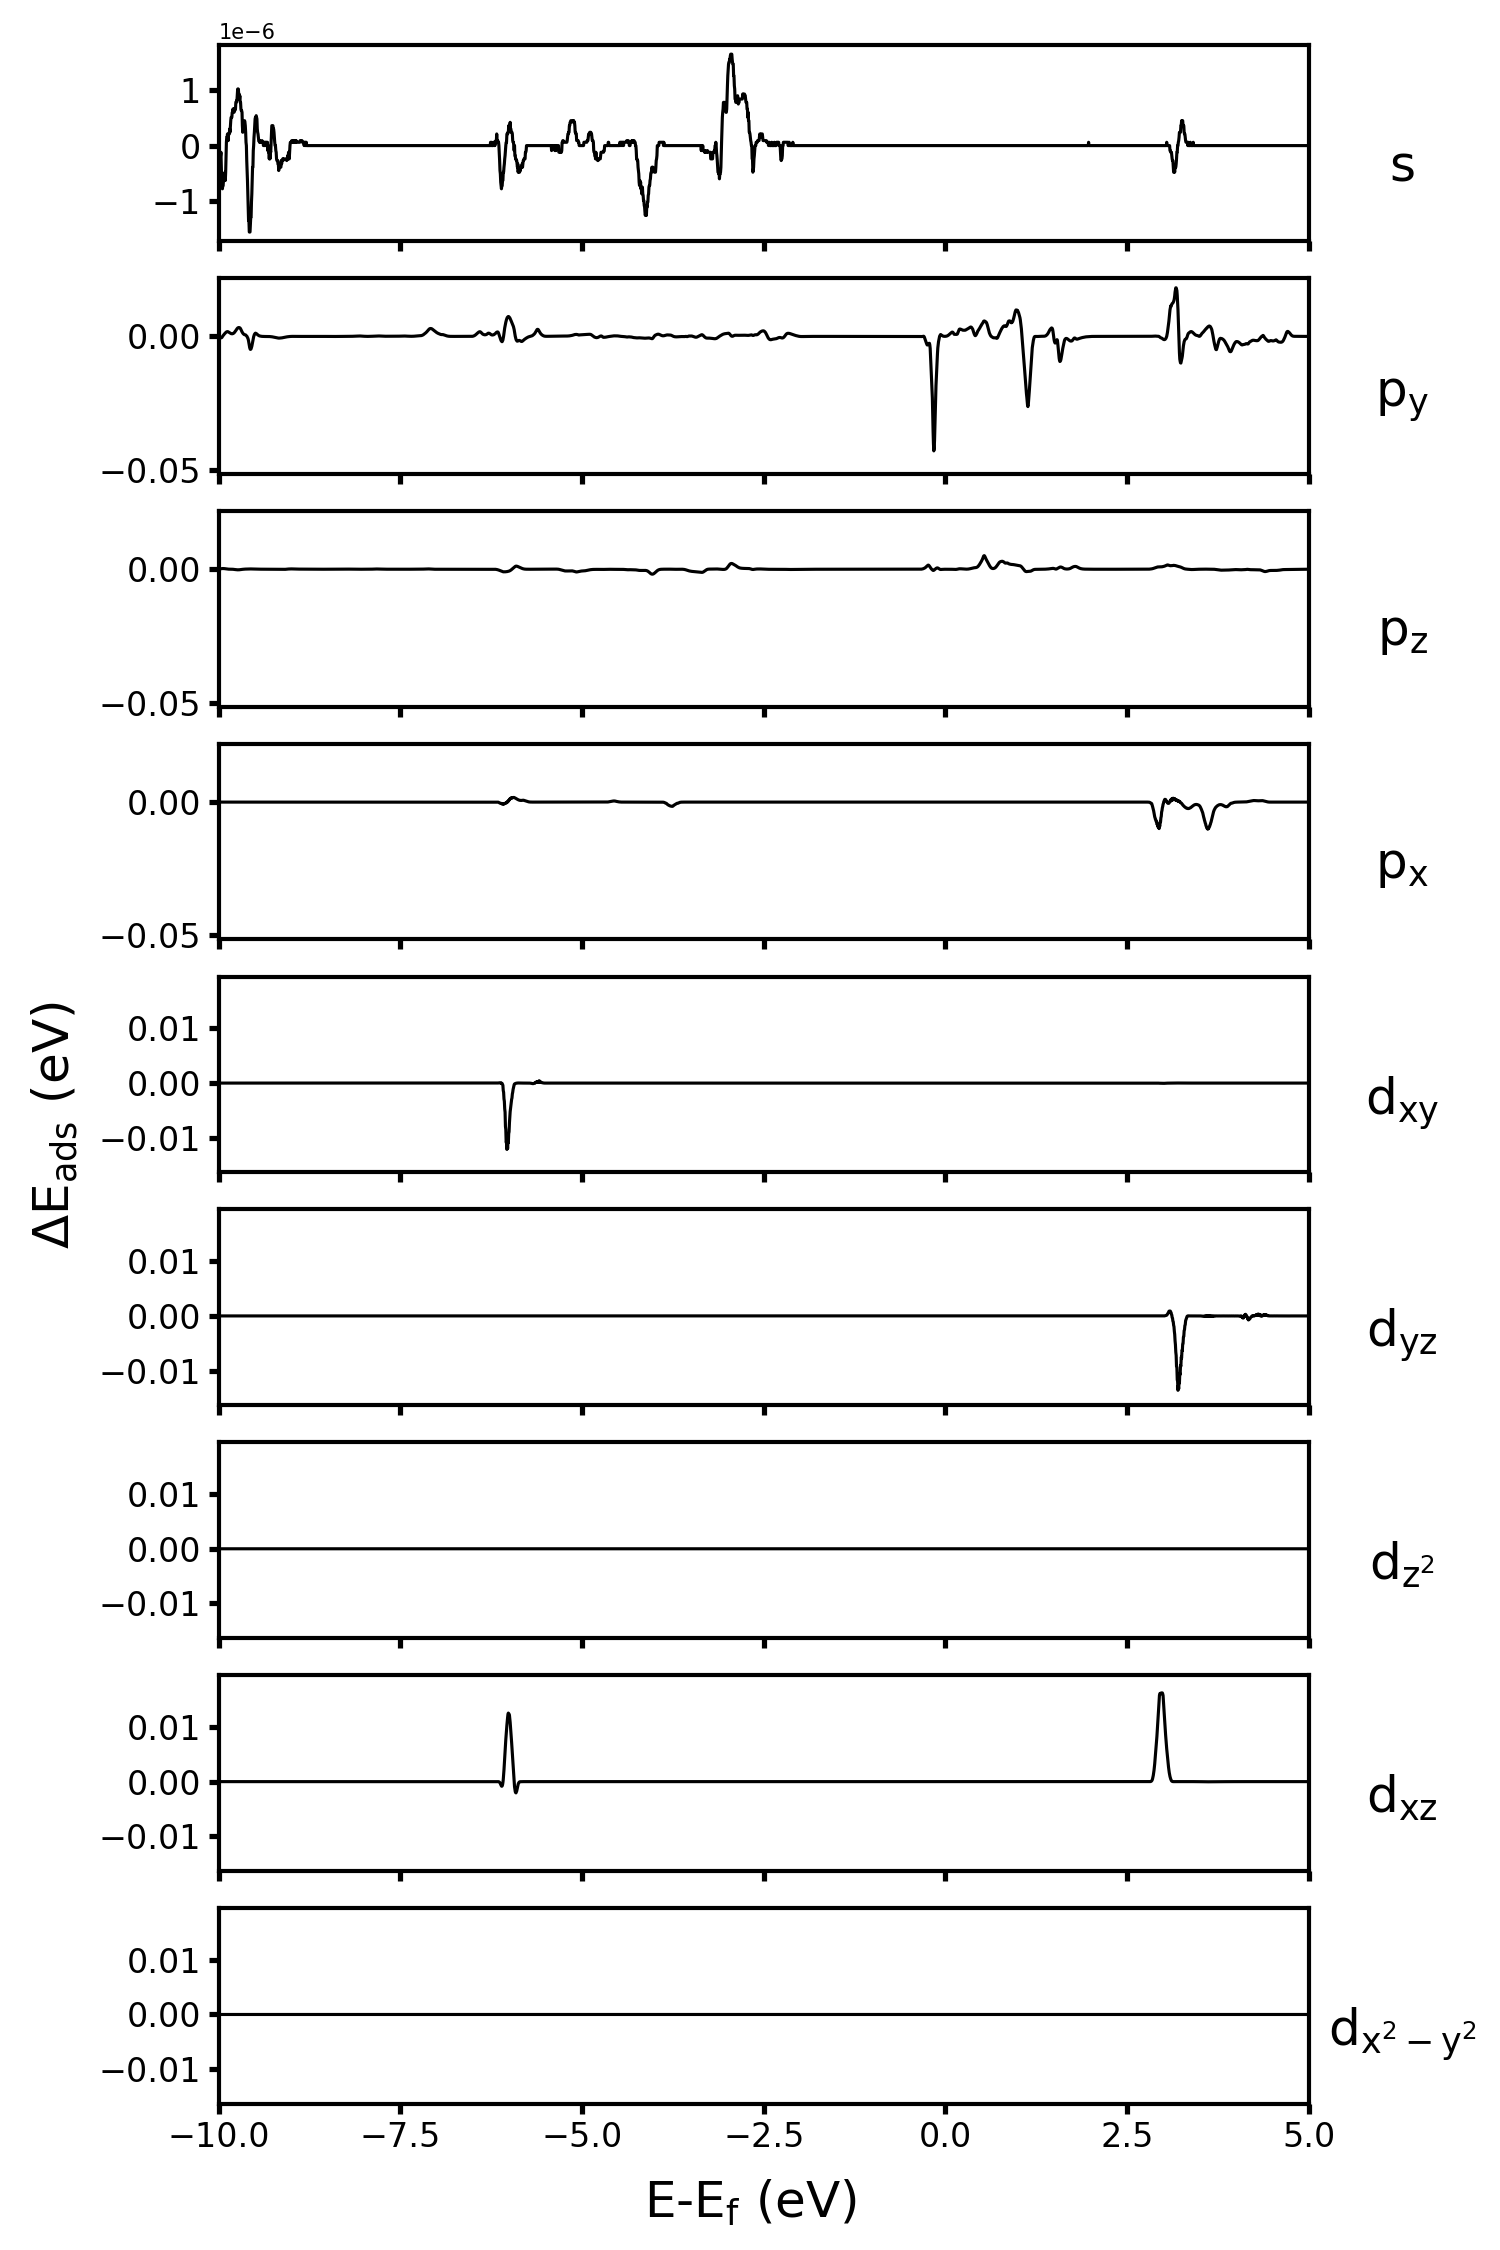
\includegraphics[width=0.6\textwidth]{supp_fig25_occl_wid11.png}
  \caption{\textbf{Occlusion Experiment with a masker width of ``11''.}
  This figure shows an occlusion experiment on the Ge atom in
  the initial state of CO adsorption on Ge@g-C\textsubscript{3}N\textsubscript{4}.}
  \label{supp_fig25:occl_wid11}
\end{figure}

% SI Figure 26: Occlusion experiment with a masker width of 21
\begin{figure}[htbp]
  \centering
  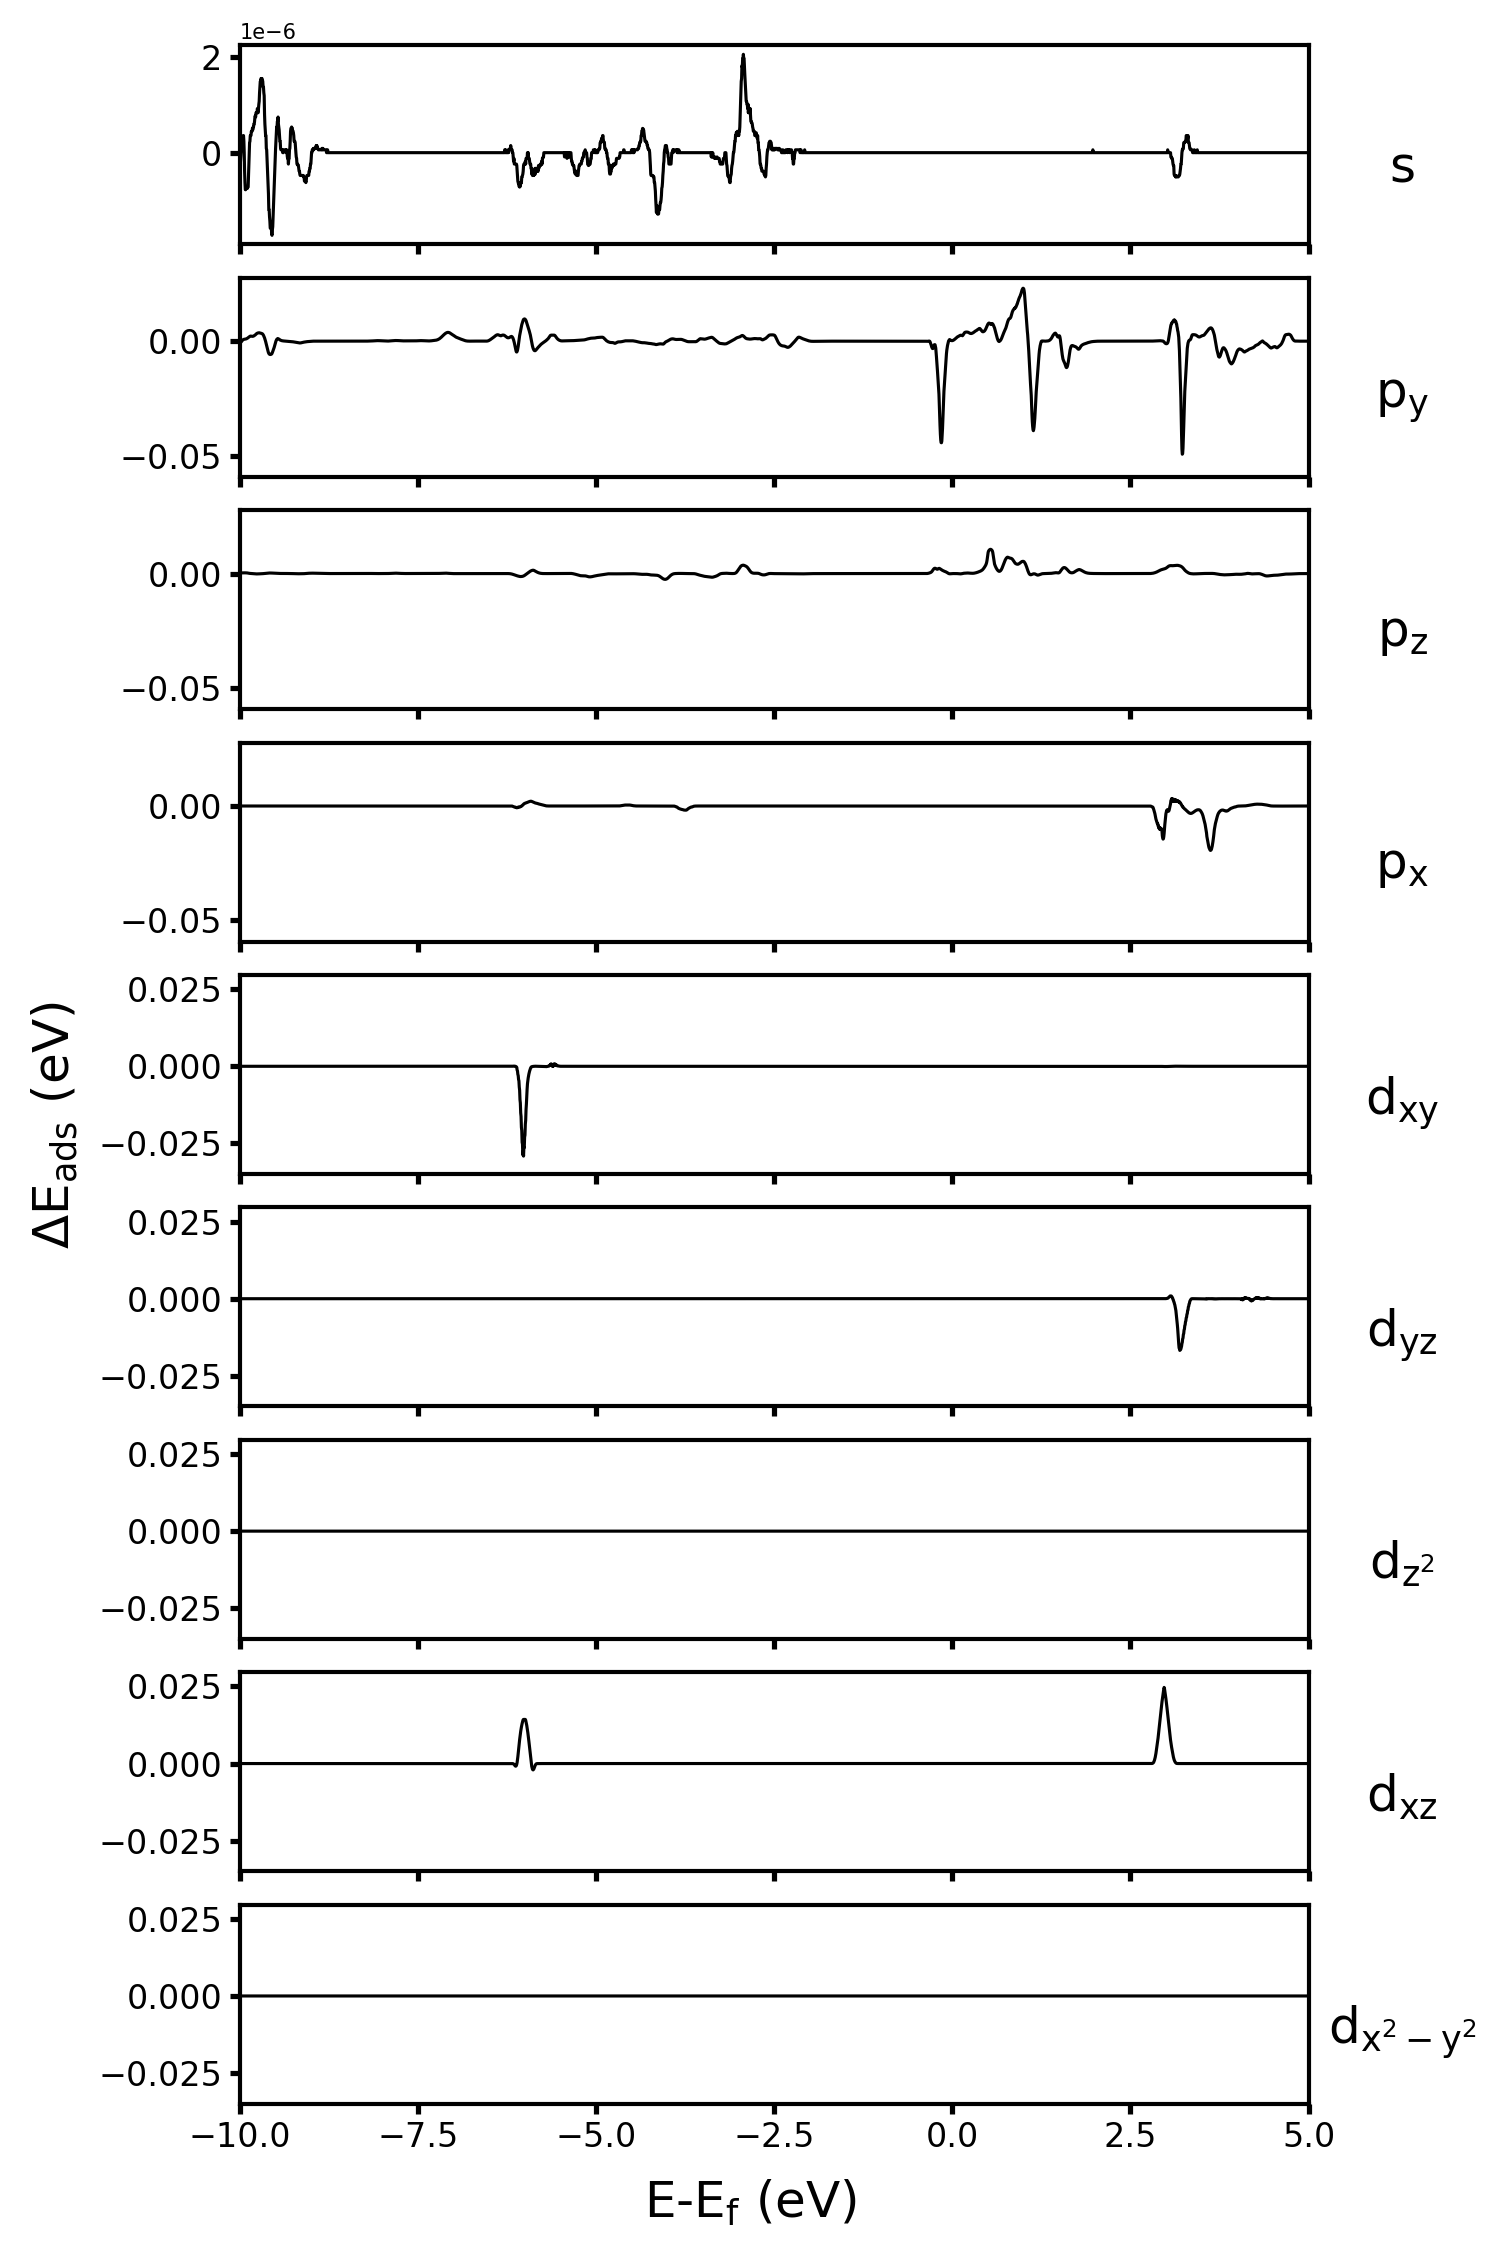
\includegraphics[width=0.6\textwidth]{supp_fig26_occl_wid21.png}
  \caption{\textbf{Occlusion Experiment with a masker width of ``21''.}
  This figure shows an occlusion experiment on the Ge atom in
  the initial state of CO adsorption on Ge@g-C\textsubscript{3}N\textsubscript{4}.}
  \label{supp_fig26:occl_wid21}
\end{figure}

% SI Figure 27: Occlusion experiment with a masker width of 31
\begin{figure}[htbp]
  \centering
  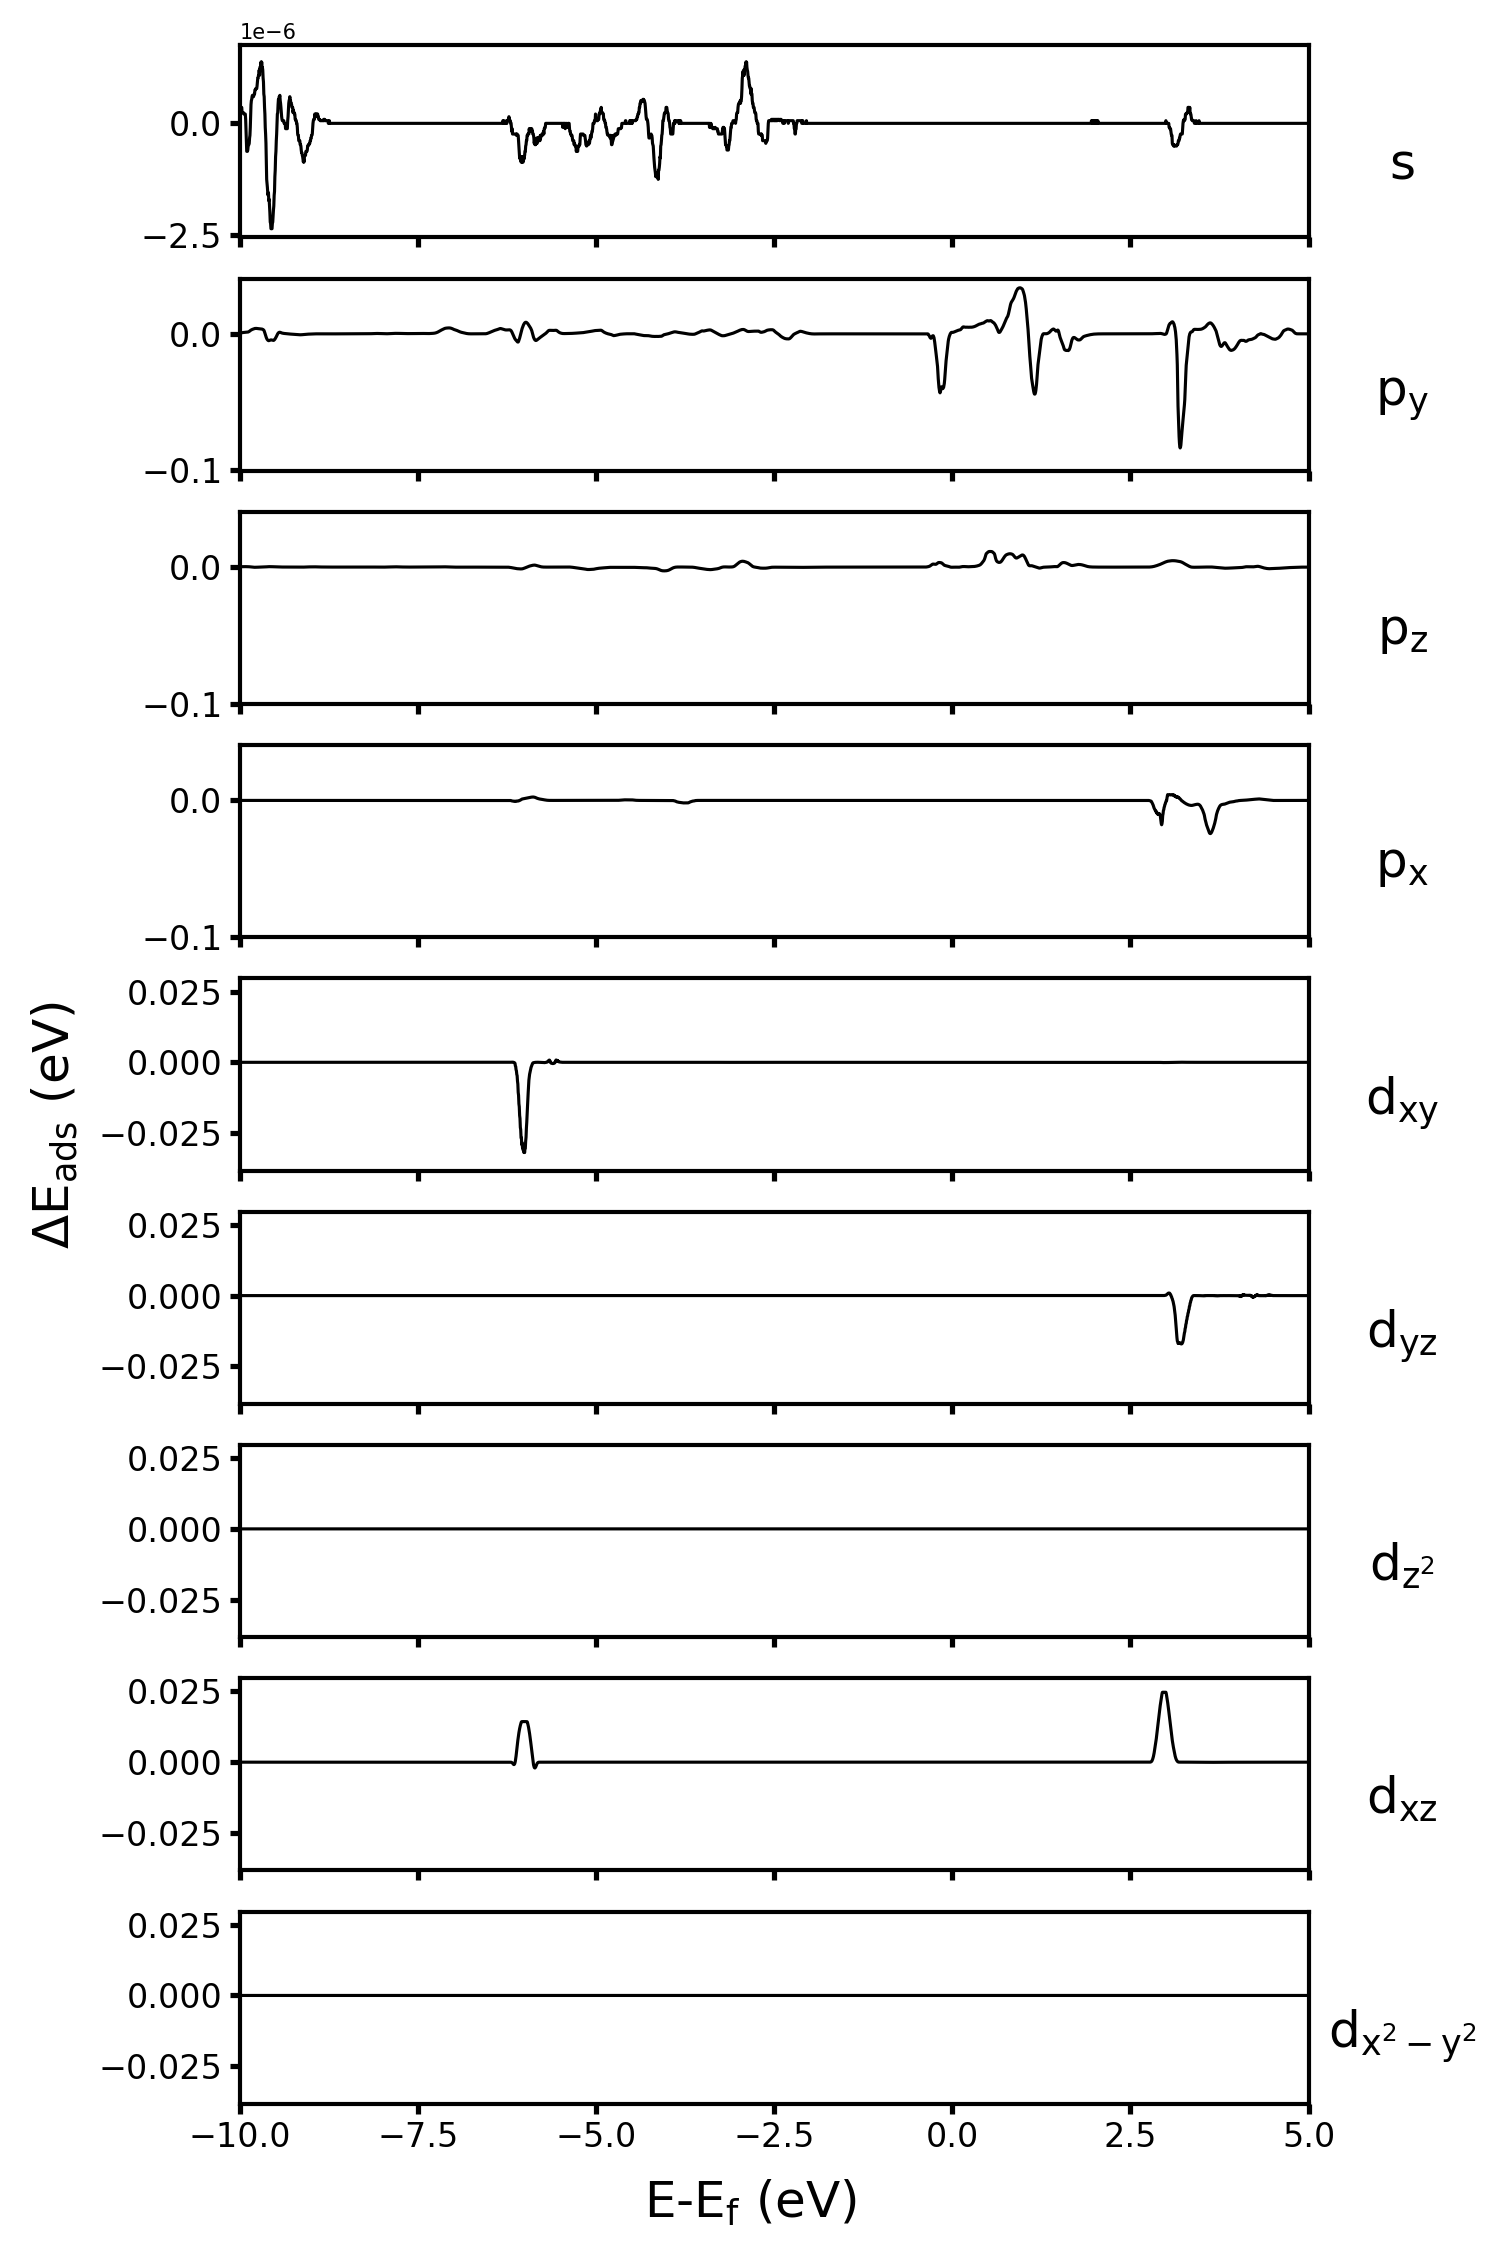
\includegraphics[width=0.6\textwidth]{supp_fig27_occl_wid31.png}
  \caption{\textbf{Occlusion Experiment with a masker width of ``31''.}
  This figure shows an occlusion experiment on the Ge atom in
  the initial state of CO adsorption on Ge@g-C\textsubscript{3}N\textsubscript{4}.}
  \label{supp_fig27:occl_wid31}
\end{figure}

% SI Figure 28: Occlusion experiment with a masker width of 41
\begin{figure}[htbp]
  \centering
  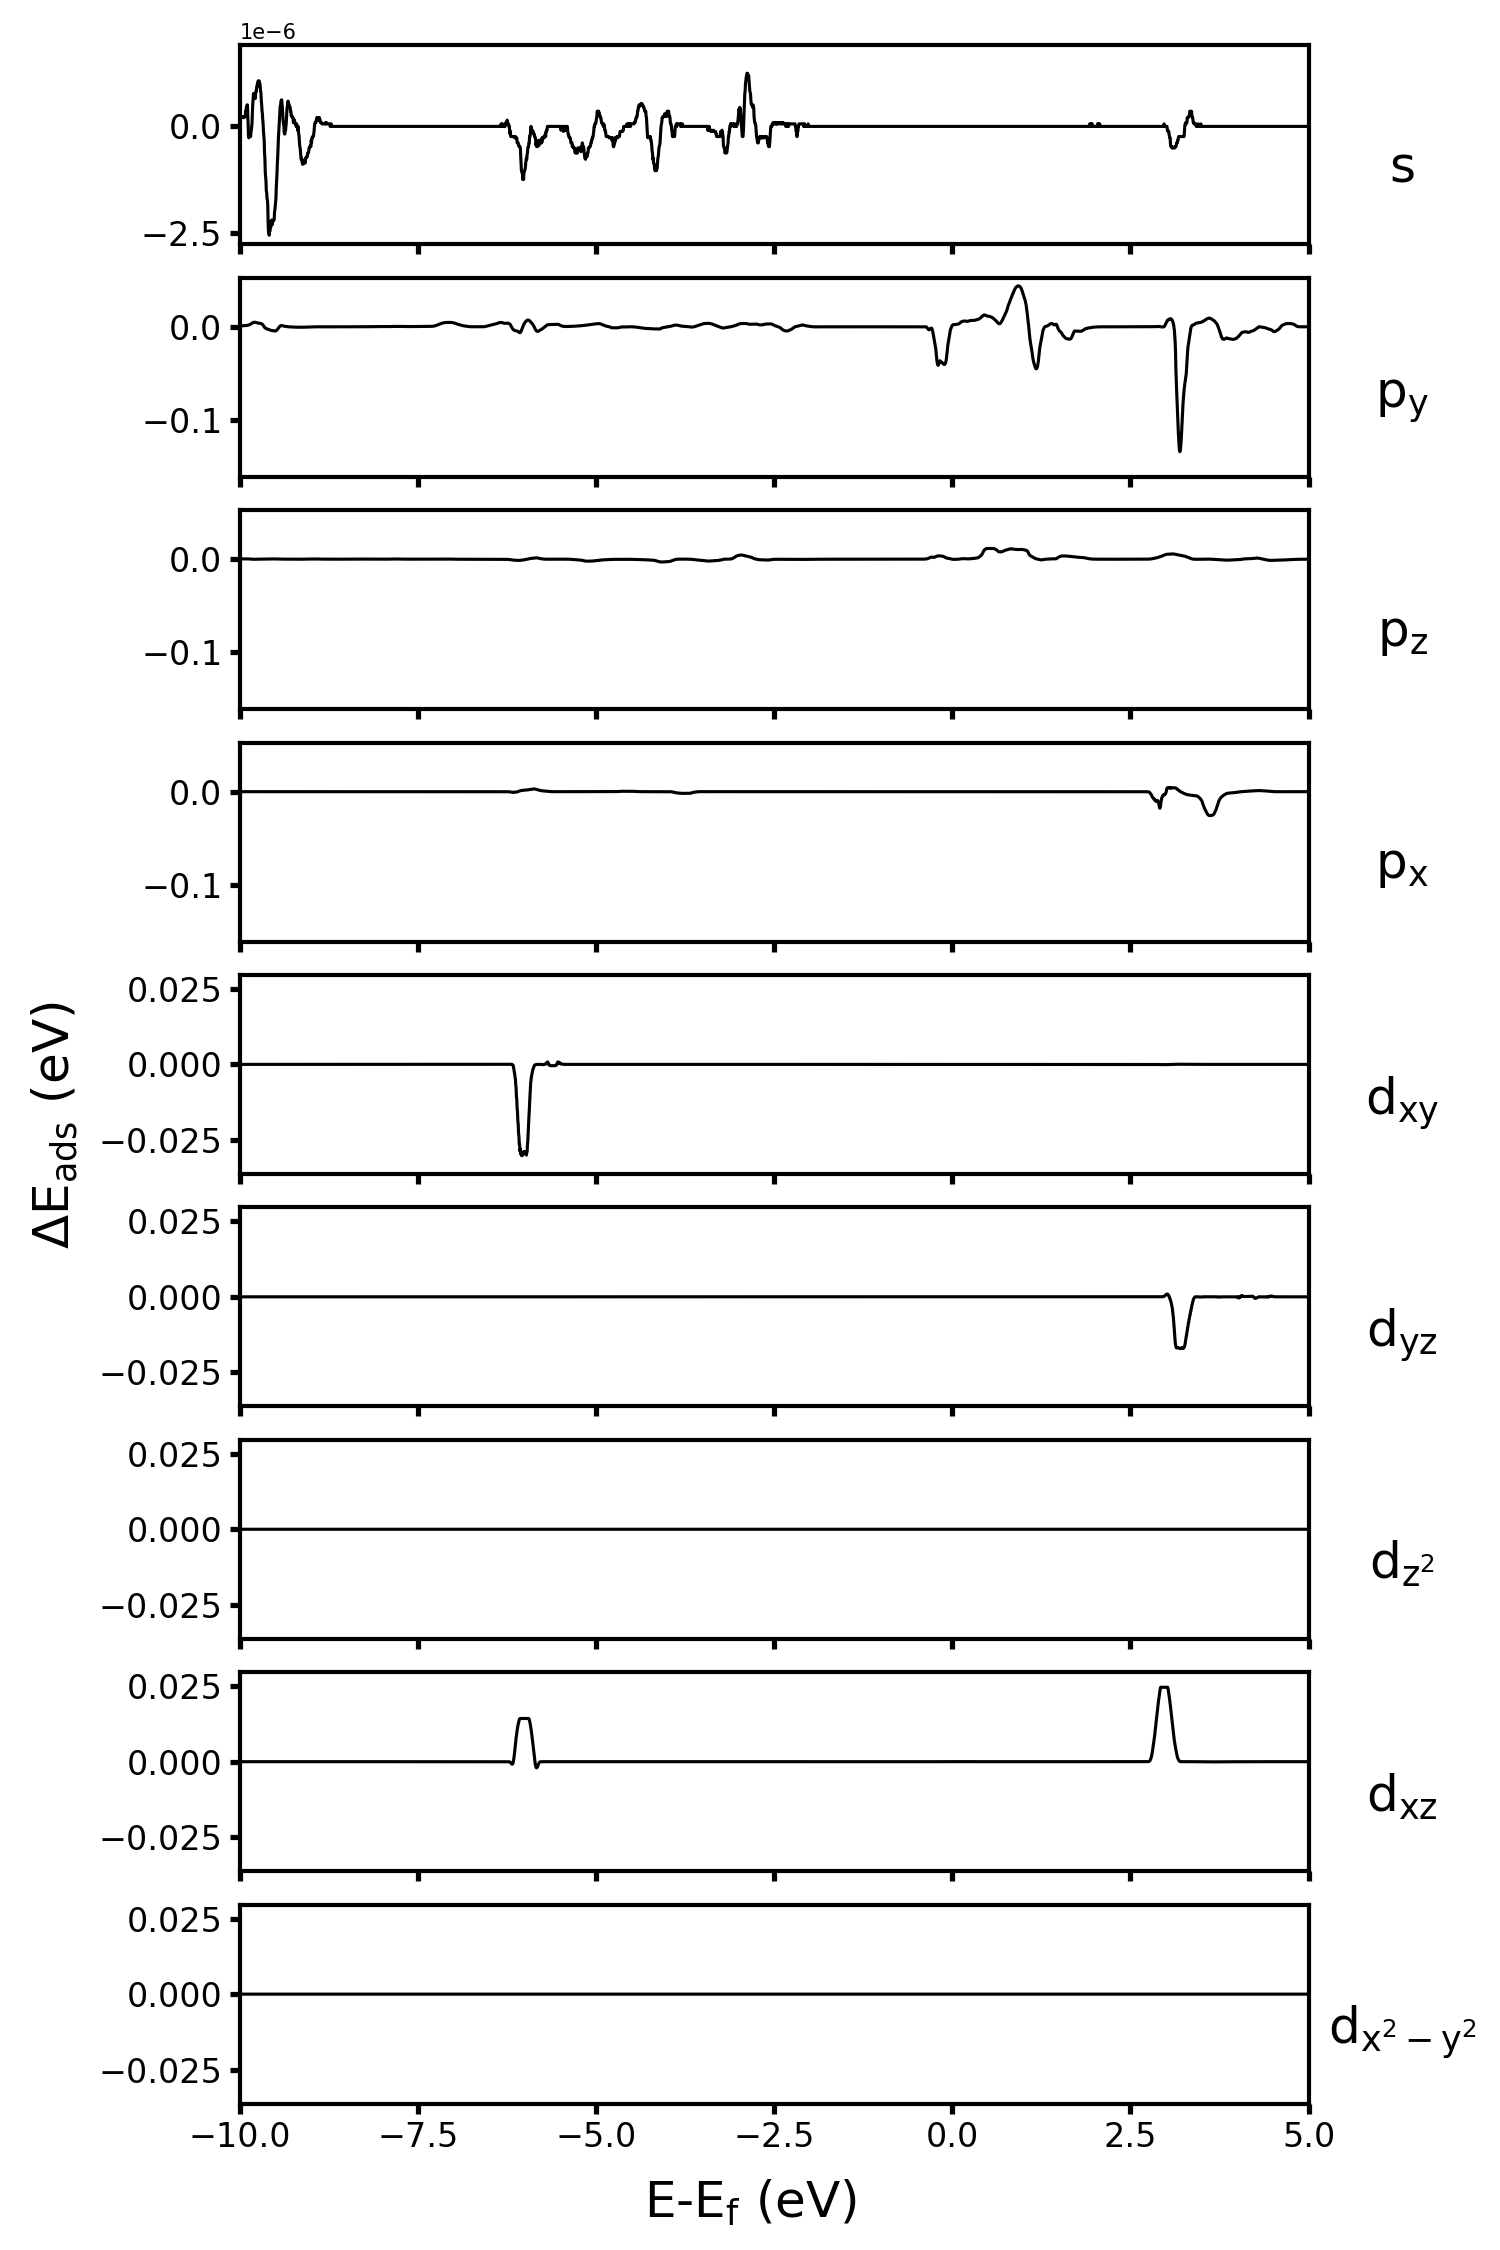
\includegraphics[width=0.6\textwidth]{supp_fig28_occl_wid41.png}
  \caption{\textbf{Occlusion Experiment with a masker width of ``41''.}
  This figure shows an occlusion experiment on the Ge atom in
  the initial state of CO adsorption on Ge@g-C\textsubscript{3}N\textsubscript{4}.}
  \label{supp_fig28:occl_wid41}
\end{figure}

% SI Figure 29: Occlusion experiment with a masker width of 51
\begin{figure}[htbp]
  \centering
  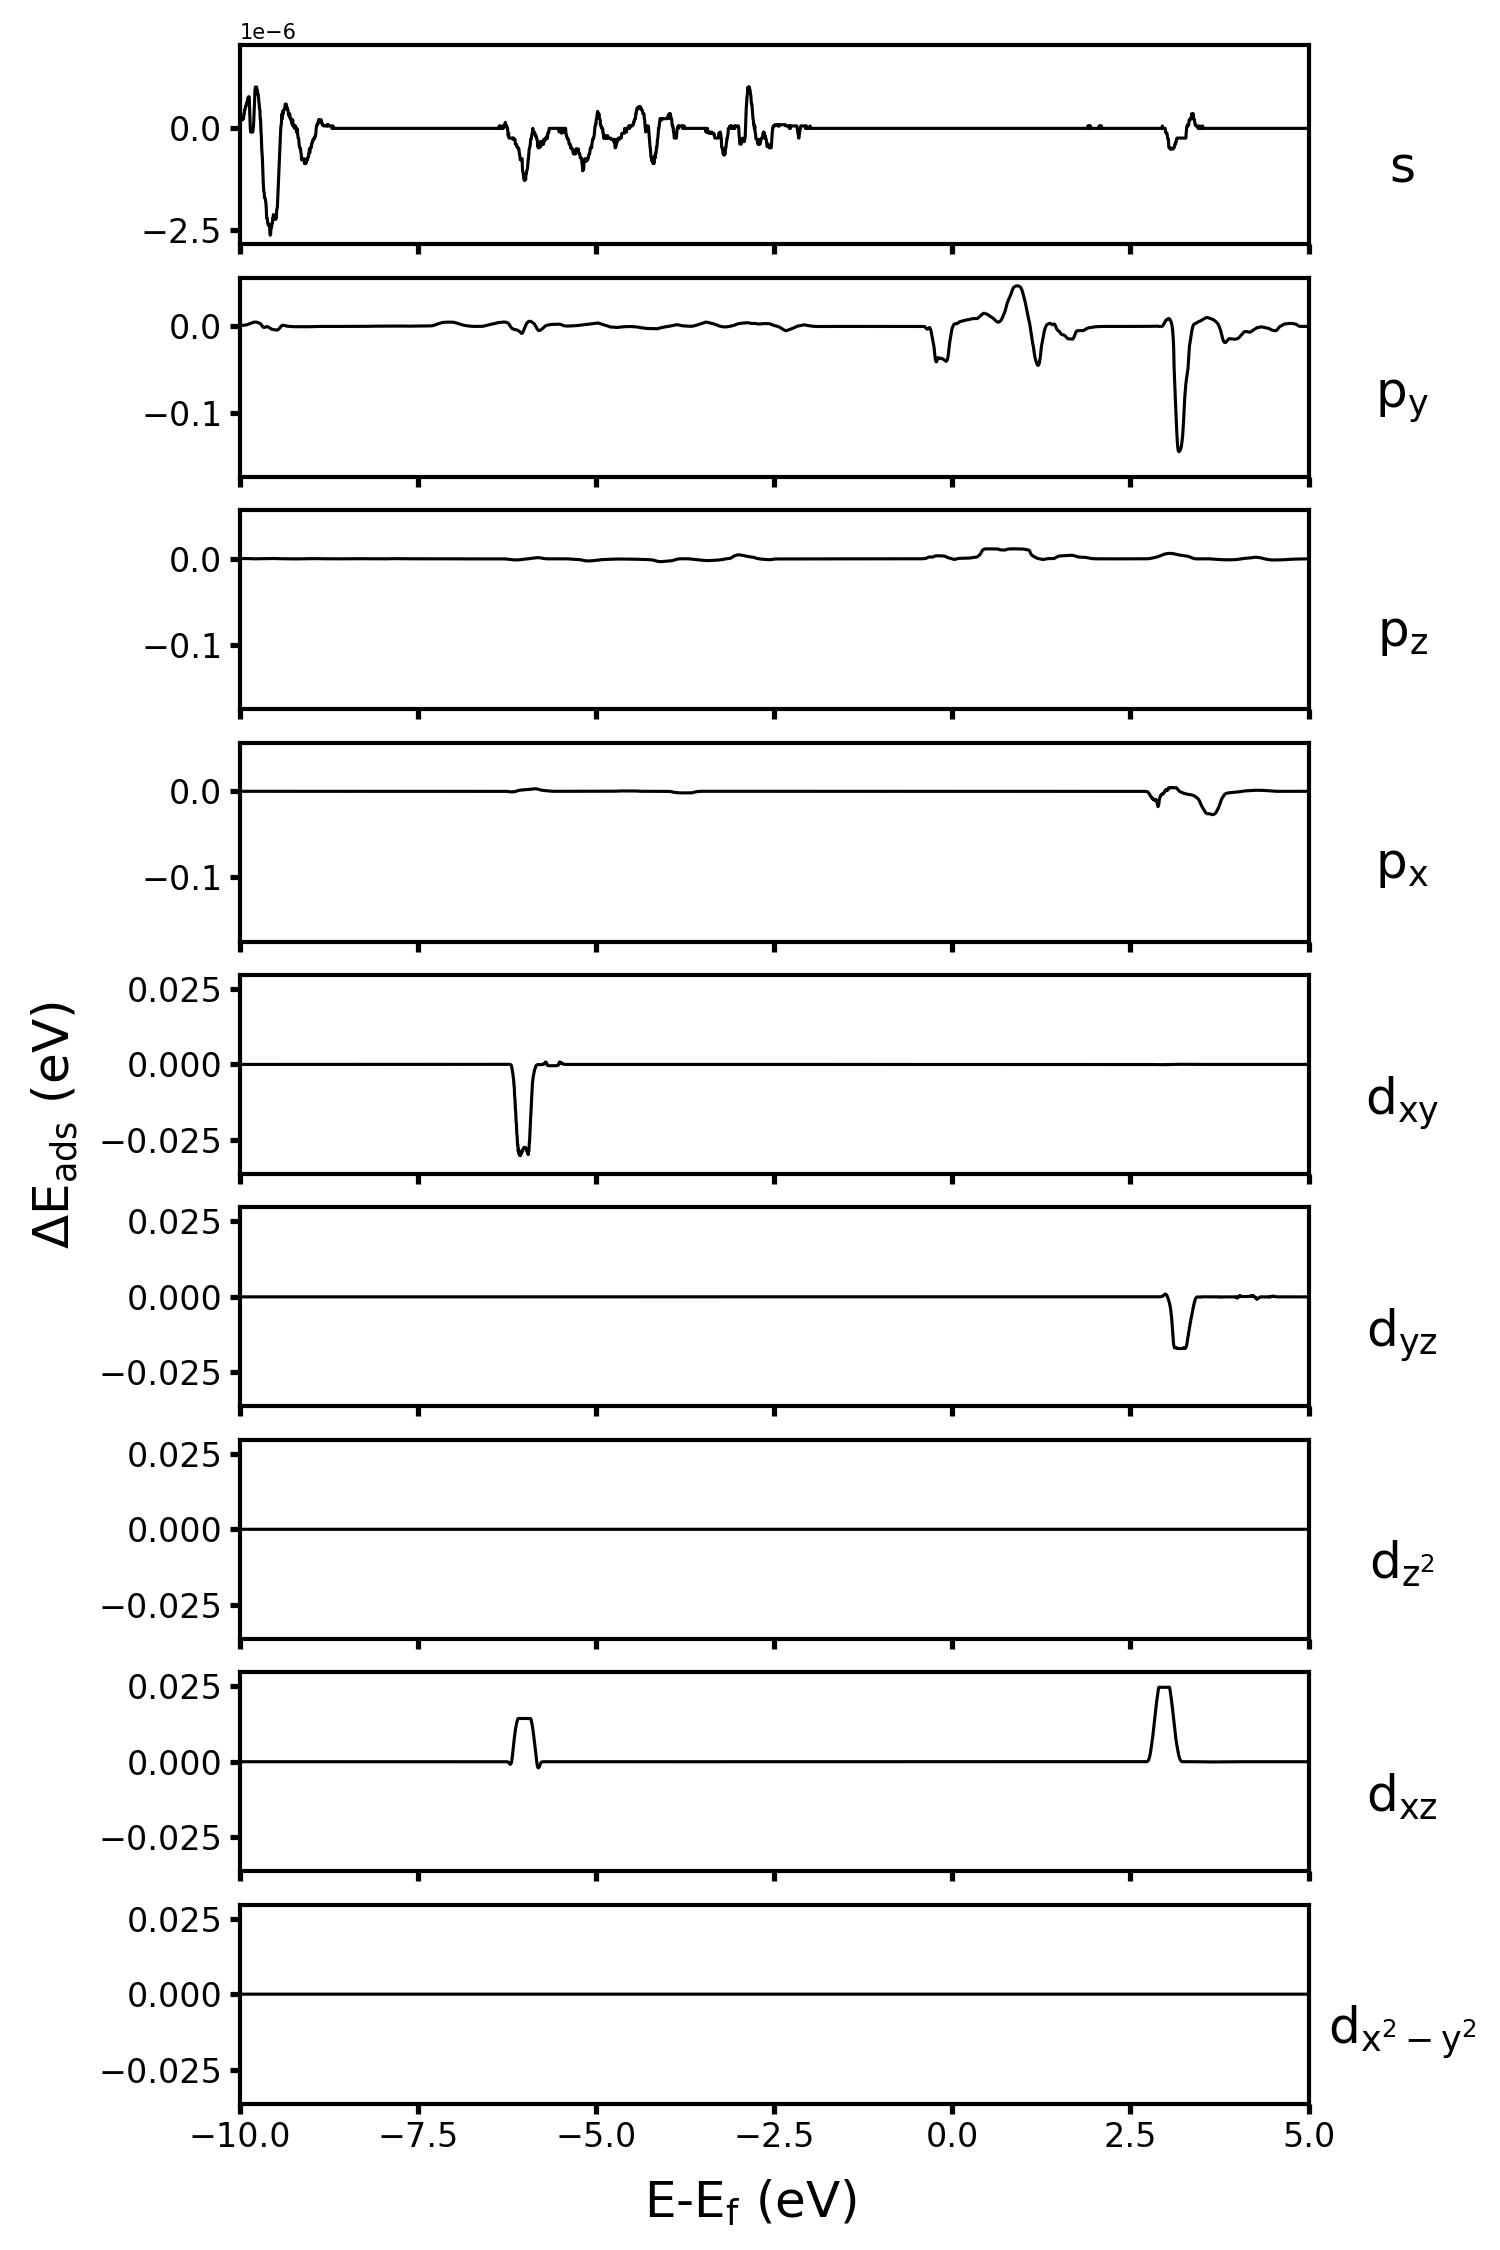
\includegraphics[width=0.6\textwidth]{supp_fig29_occl_wid51.png}
  \caption{\textbf{Occlusion Experiment with a masker width of ``51''.}
  This figure shows an occlusion experiment on the Ge atom in
  the initial state of CO adsorption on Ge@g-C\textsubscript{3}N\textsubscript{4}.}
  \label{supp_fig29:occl_wid51}
\end{figure}

\subsection{Shifting experiment}
\label{supp_sec3.6_shifting}

% SI Figure 30: Illustration of the eDOS shifting experiment
\begin{figure}[htbp]
  \centering
  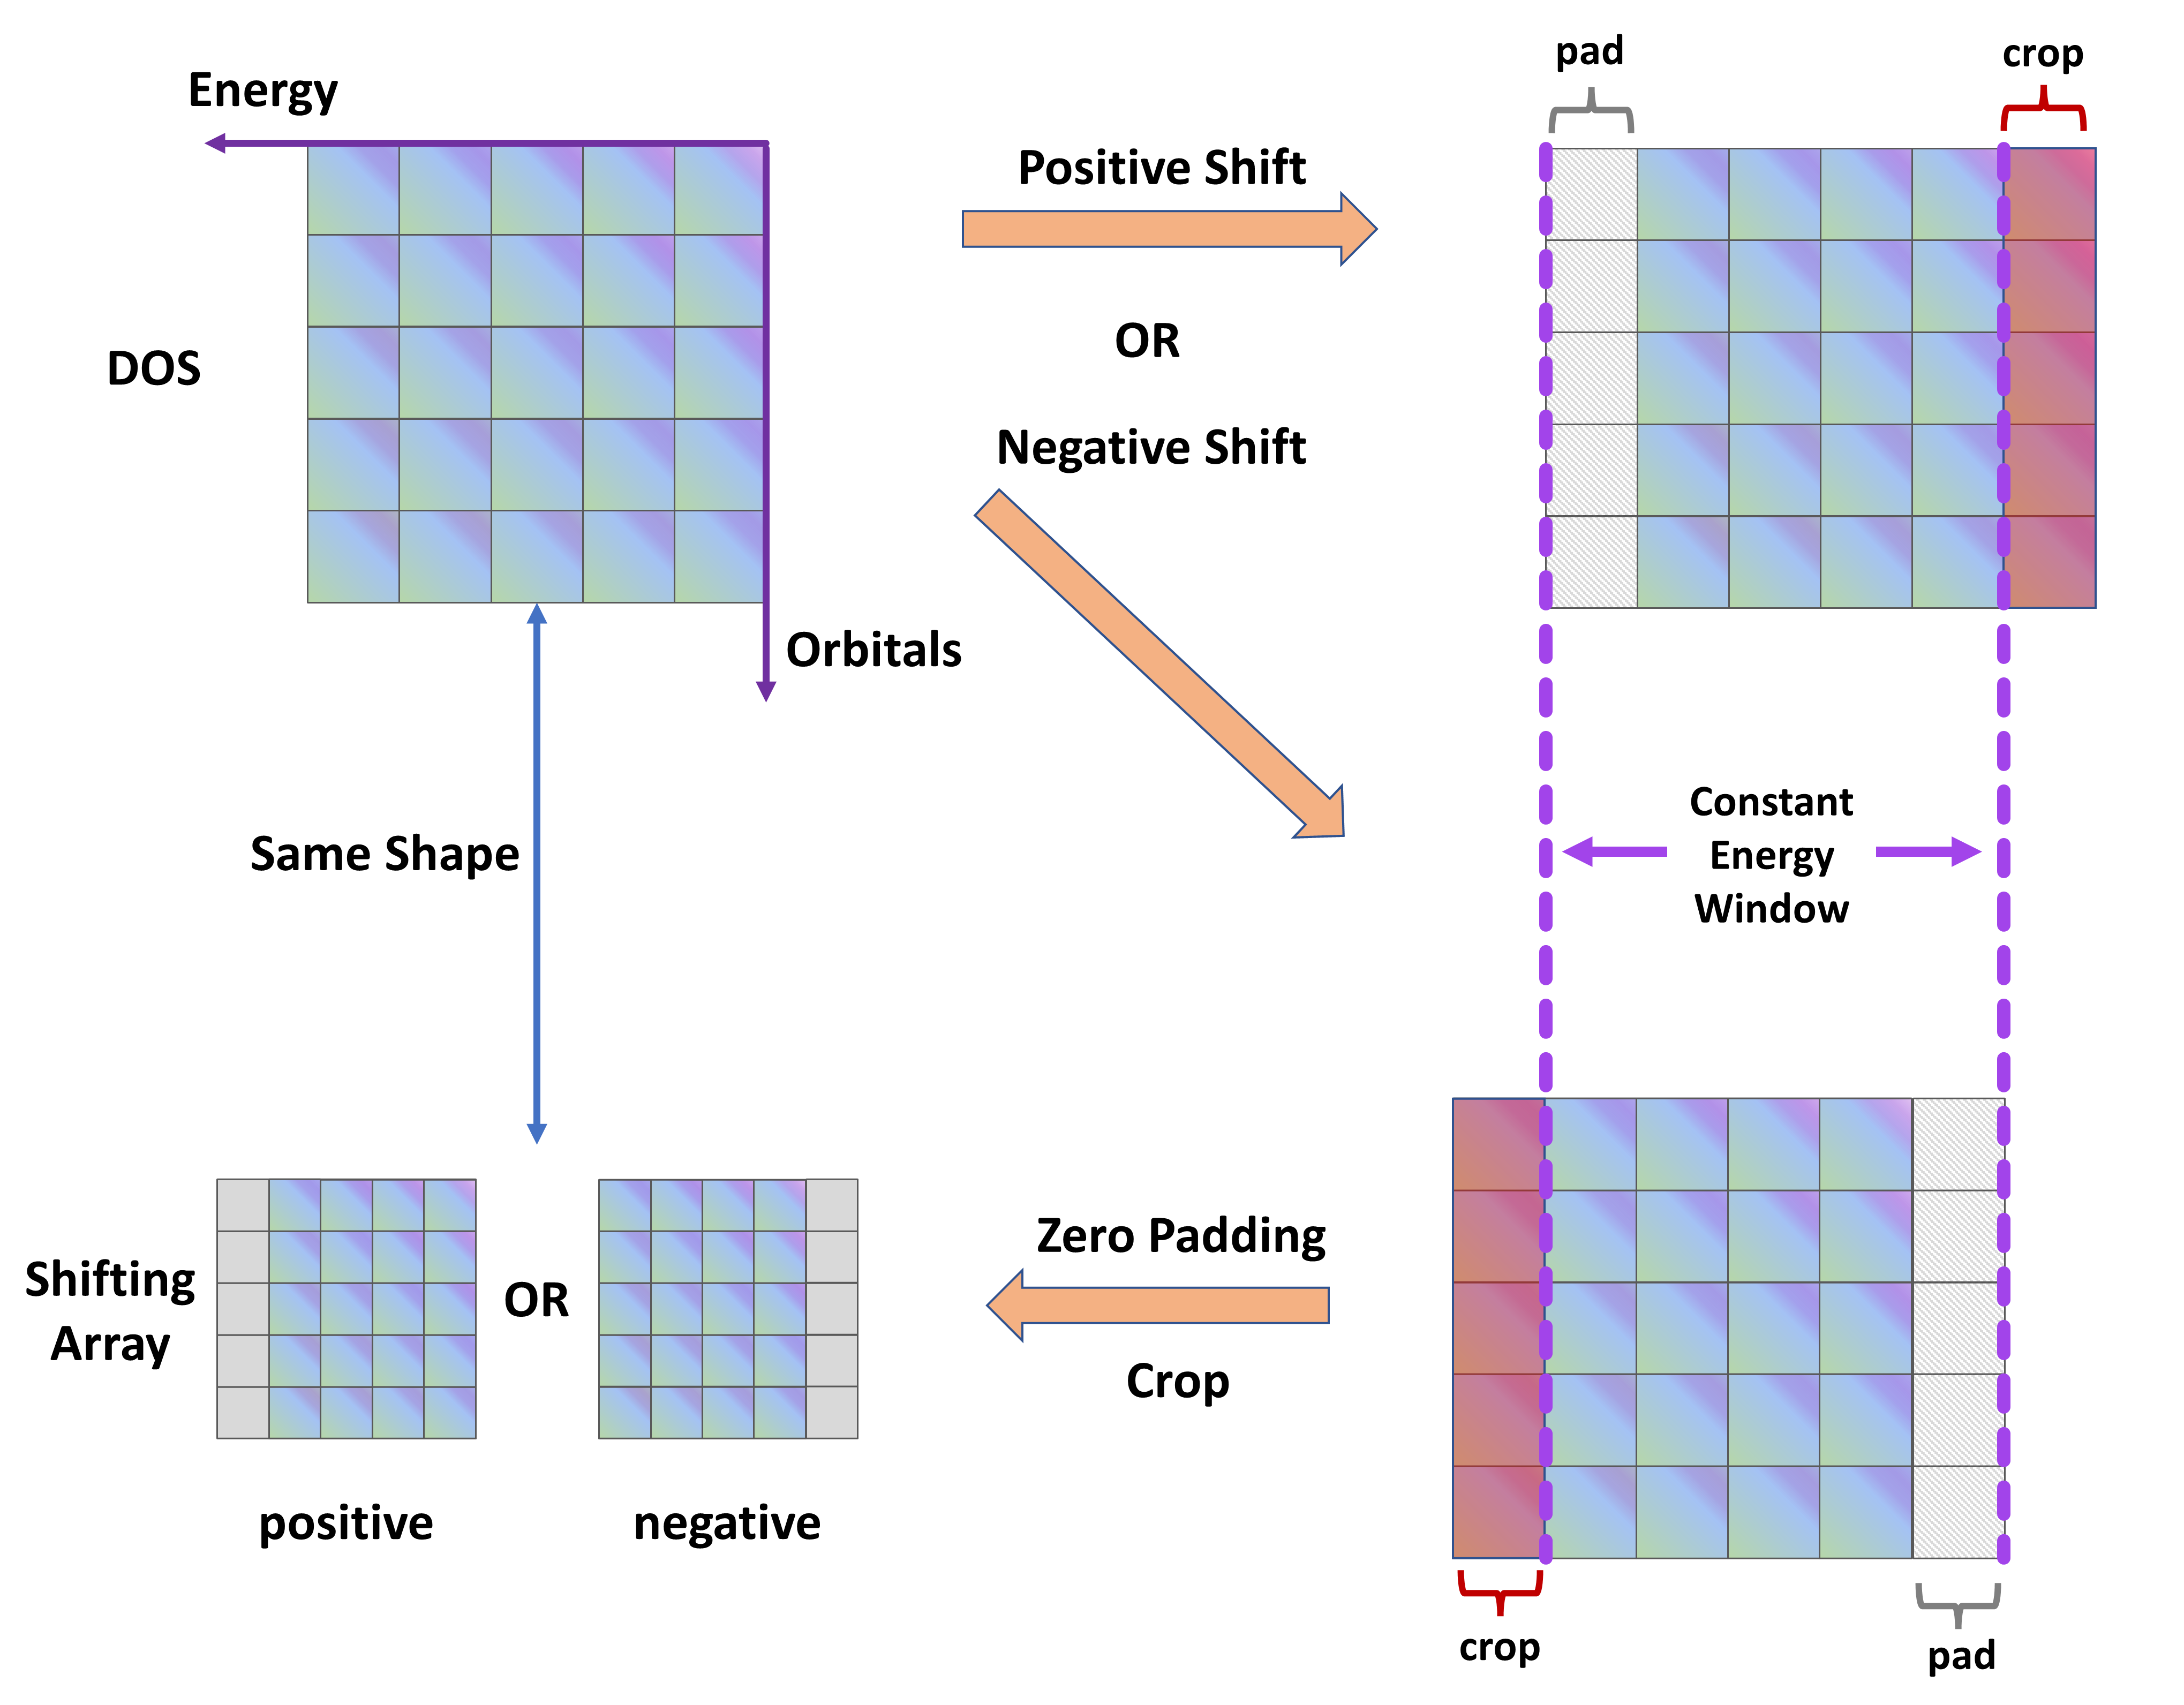
\includegraphics[width=\textwidth]{supp_fig30_shifting.png}
  \caption{\textbf{Illustration of the eDOS shifting experiment.}
  This figure illustrates the sequential stages of the shifting experiment.
  Initially, the input eDOS array is shifted along the Energy axis.
  Subsequently, it undergoes zero-padding and cropping,
  ensuring a consistent shape based on the shifting direction, to match the input eDOS array.
  The resulting shifted array is then processed by the CNN model to
  assess the disturbance in adsorption energy caused by the shifting operation.}
  \label{supp_fig30:shifting}
\end{figure}

% SI Figure 31: Shifting experiment on p orbital
\begin{figure}[htbp]
  \centering
  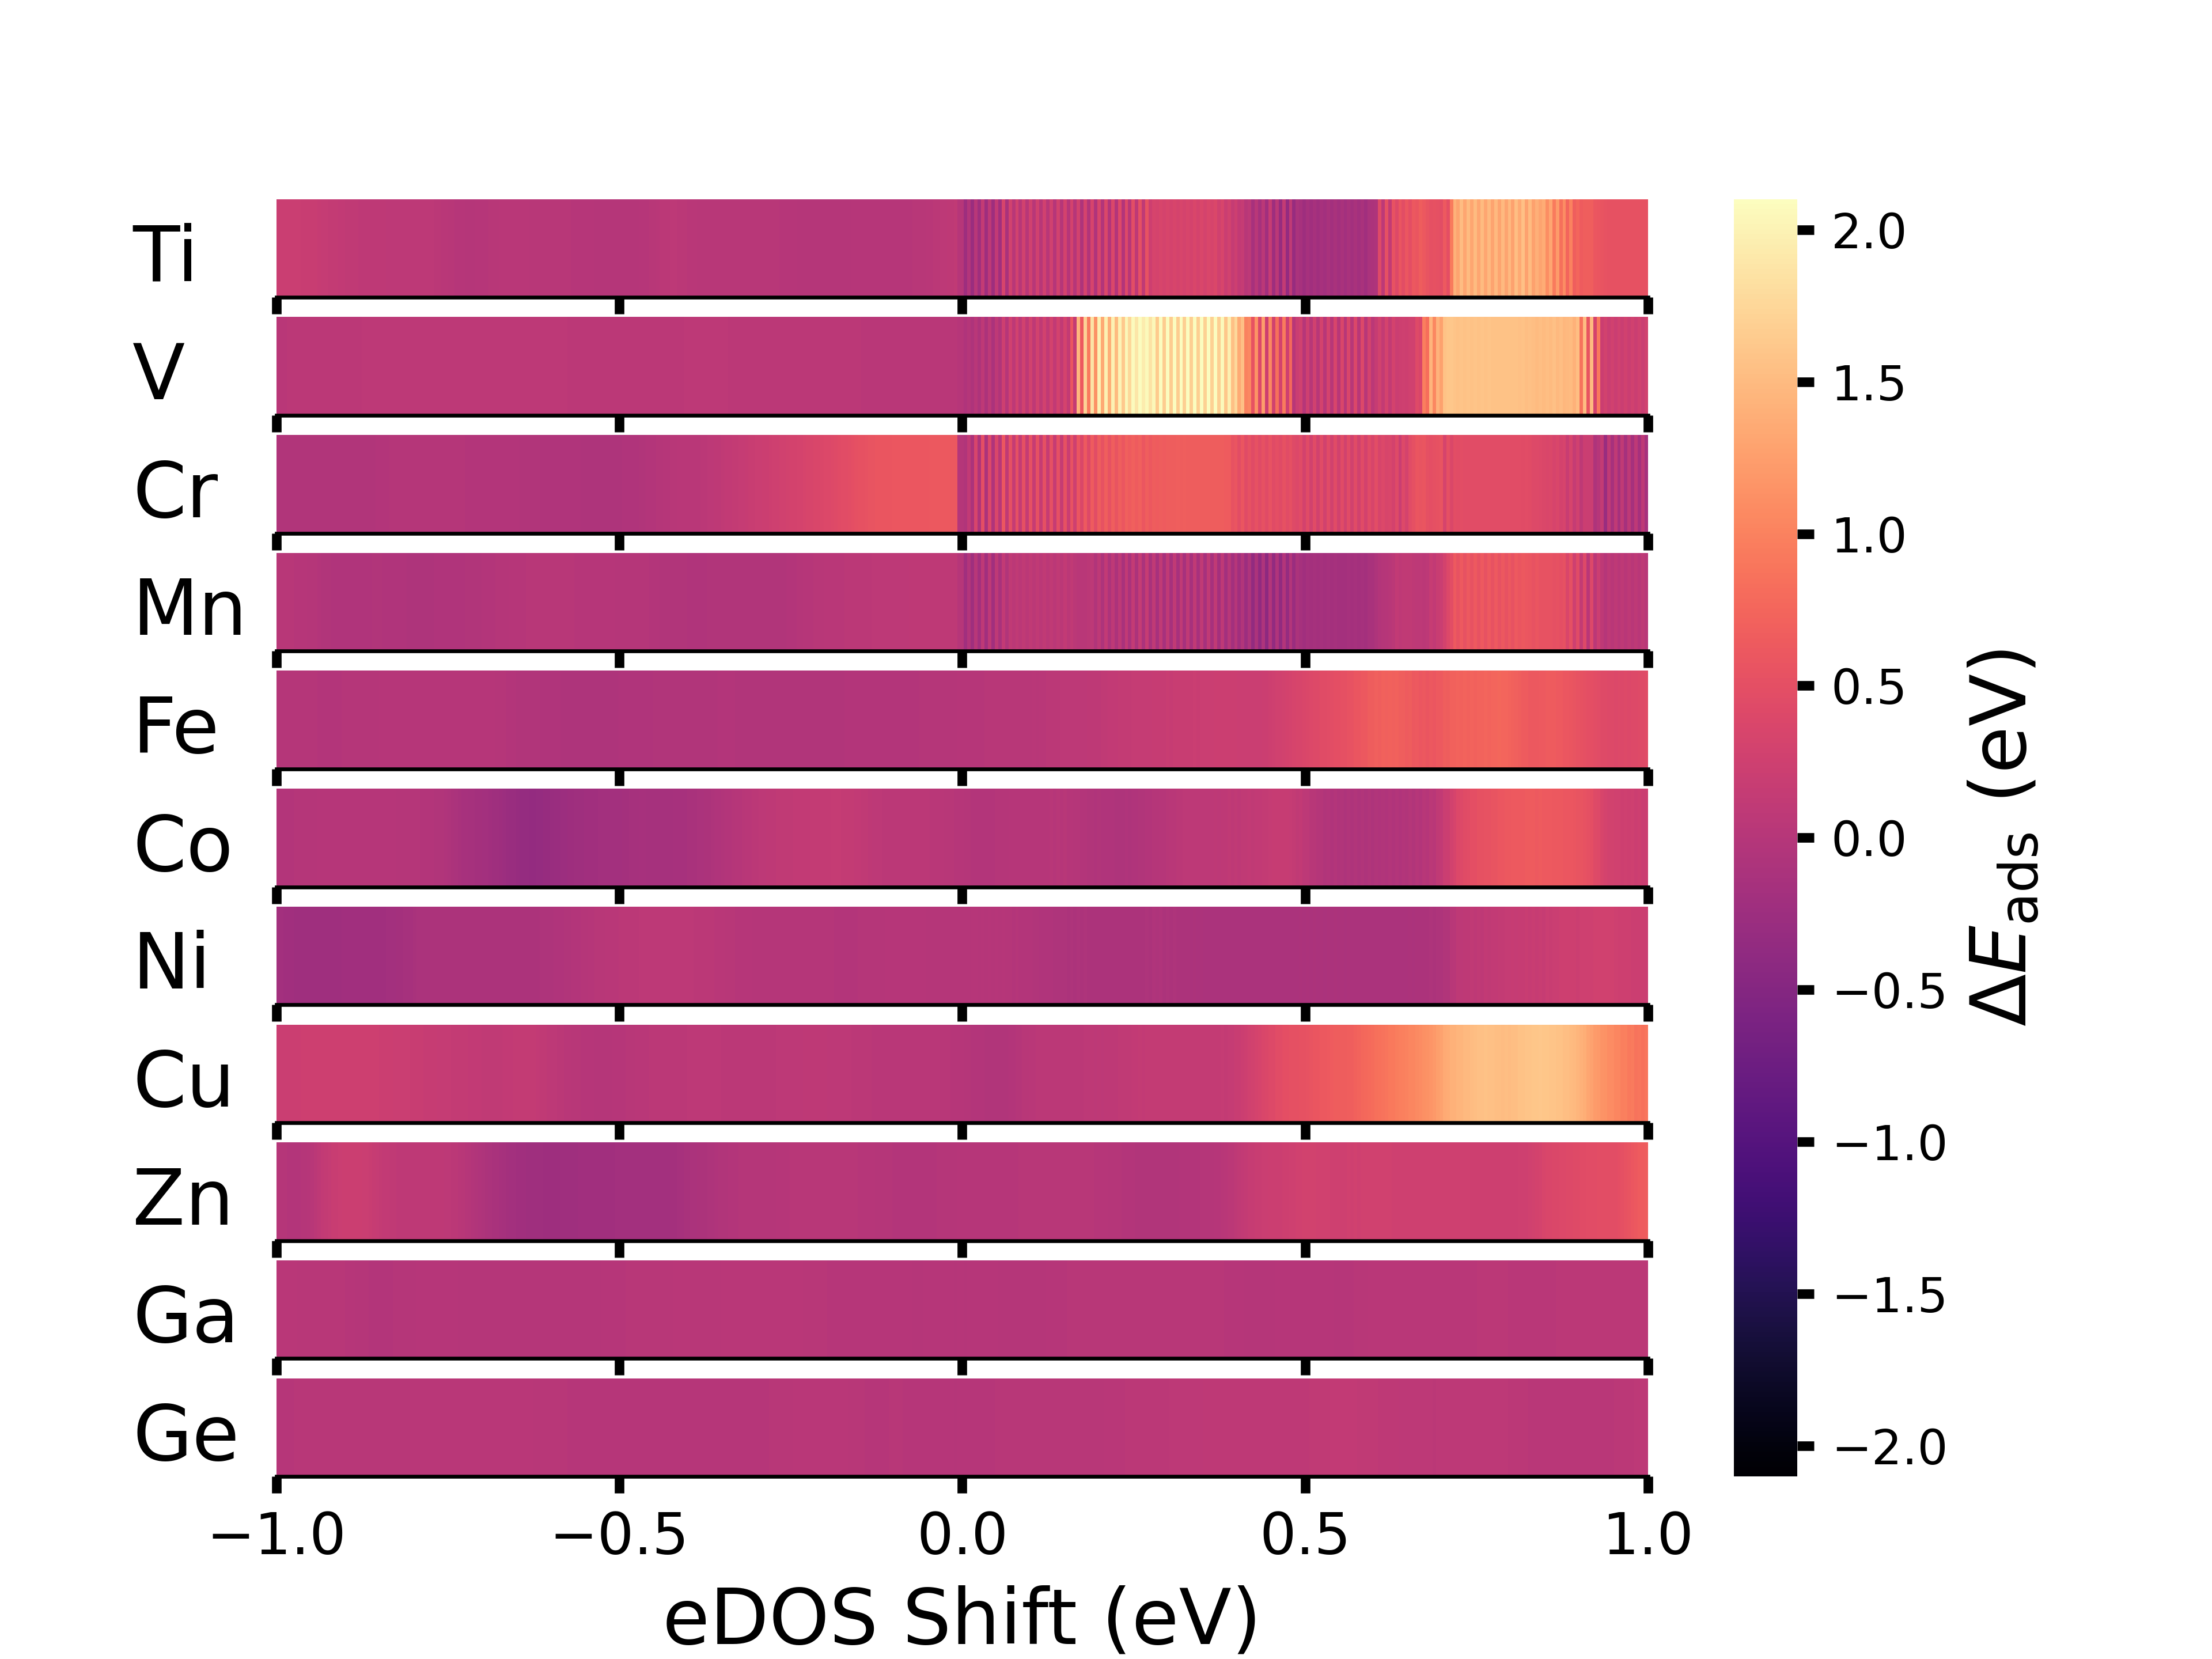
\includegraphics[width=0.75\textwidth]{supp_fig31_p_shifting.png}
  \caption{\textbf{Shifting experiment on p orbital.}
  Effect of orbital shifting on CO adsorption energy, predicted by the CNN model,
  for single metal atom catalysts supported on g-C\textsubscript{3}N\textsubscript{4}.
  The perturbations caused by shifting of entire p orbital are presented.
  The shifting step size corresponds to the energy resolution of the eDOS, set at 0.005 eV in this study.
  A positive eDOS shift indicates a shift towards higher energy levels, and vice versa.}
  \label{supp_fig31:p_shifting}
\end{figure}
